\documentclass[10pt]{article}
\usepackage[T1]{fontenc}
\usepackage[utf8]{inputenc}
\usepackage{lmodern}
\usepackage[margin=1in]{geometry}
\usepackage{amsmath,amssymb}
\usepackage{microtype}
\usepackage{parskip}
\linespread{1.08}
\usepackage{booktabs}
\usepackage{graphicx}
\usepackage{float}
\usepackage{adjustbox}
\usepackage[dvipsnames]{xcolor}
\usepackage{hyperref}
\hypersetup{colorlinks=true, linkcolor={Maroon}, urlcolor={Blue}}
\setcounter{secnumdepth}{-\maxdimen} % no section numbering
\providecommand{\tightlist}{%
  \setlength{\itemsep}{2pt}\setlength{\parskip}{0pt}}

\title{CS683 PA2: Final Report}
\author{\textbf{Team: Huffman} \\[3pt]
  Shaik Awez Mehtab (23b1080), Satyam Sinoliya (23b0958), \\
  Gautam Siddarth (23b0957), Mohana Evuri (23b1017)}
\date{}

\begin{document}
\maketitle
\section{Task 1: Stride Pattern Prefetcher (SPP)}

\subsection{Setup}

\begin{itemize}
\tightlist
\item Every run: 25M warmup + 25M simulated instructions on the 3 given traces, ChampSim built with GCC 7 (as asked), LRU everywhere unless stated.
\item Accuracy is ChampSim's L1D accuracy (useful / prefetches sent to the L2C). Coverage is the fraction of L1D load misses that prefetching removes.
\item Everything can be rerun with \texttt{scripts/task\{1,2,3\}.sh all}; raw outputs are in \texttt{results/}, plots in \texttt{plots/}.
\end{itemize}

\subsection{Task 1A: IP-stride}

\texttt{ip\_stride.l1d\_pref} keeps a 24-entry table (LRU, tagged by the low 8 bits of the IP). Each entry has the last line that IP touched and the last stride. On an access it computes the new stride, and if it's the same as the stored one (seen twice in a row) it prefetches \texttt{line + k*stride} for k = 1..3, within the 4 KB page. So it only catches constant strides, a sequence like +1, +2, +2, +2, +3 breaks it on most accesses.


\subsection{Task 1B: SPP (\texttt{prefetcher/spp.l1d\_pref})}

\subsubsection{Tables}

\begin{itemize}
\tightlist
\item IP table (64 entries, LRU): per-IP last line, last stride, a 2-bit stride confidence and a 12-bit signature, which is a hash of that IP's recent strides (\texttt{sig = (sig $<$$<$ 3 \textasciicircum{} stride) \& 0xFFF}).
\item Pattern table (1024 entries): shared, indexed by \texttt{signature \textasciicircum{} IP bits}, gives the stride that followed that history (+ 2-bit confidence). Mixing in IP bits keeps patterns mostly per IP.
\item Recent-prefetch filter (32 lines). Without it a stream sends the same lines again on every access.
\item Accuracy checker (128 lines): the last lines SPP prefetched, for the throttle (below).
\end{itemize}

\subsubsection{On every demand load/store}

\begin{itemize}
\tightlist
\item SPP updates the stride confidence, trains the pattern table at the old signature with the new stride, and folds the stride into the signature.
\item Uniform first: if the stride is repeating, SPP prefetches \texttt{line + k*stride}.
\item It falls back to non-uniform when the pattern table confidently predicts a \emph{different} next stride (i.e. the run of equal strides is about to end), or when there's no uniform stride at all. Non-uniform walks the pattern table: predict a stride, prefetch, fold it into a speculative signature, repeat.
\item Prefetches never cross the page, and the walk stops at the first unconfident prediction.
\end{itemize}

\subsubsection{Throttling}

SPP has its own accuracy checker: it remembers the last 128 lines it prefetched, and counts a prefetch as useful when a later demand access hits one of them. Every 256 issued prefetches, it computes useful / issued for that window and sets the degree from it:


\begin{center}
\begin{adjustbox}{max width=\linewidth}
\begin{tabular}{@{}lrrrr@{}}
\toprule
\textbf{window accuracy} & \textbf{$<$ 25\%} & \textbf{25-50\%} & \textbf{50-75\%} & \textbf{$\geq$ 75\%} \\
\midrule
degree & 1 & 2 & 4 & 6 \\
\bottomrule
\end{tabular}
\end{adjustbox}
\end{center}

Before the real traces, we checked it on a synthetic trace (one +2 stream, one +1,+2,+2,+2,+3 stream). IP-stride turned 37\% of the L1D load misses into hits, SPP turned 87\% into hits at 83\% accuracy.


\subsection{Results}

\begin{center}
\begin{minipage}[t]{0.48\linewidth}\centering
\textbf{IPC}\\[3pt]
\begin{adjustbox}{max width=\linewidth}
\begin{tabular}{@{}lrrr@{}}
\toprule
\textbf{config} & \textbf{trace1} & \textbf{trace2} & \textbf{trace3} \\
\midrule
No-prefetch & 0.2322 & 0.2513 & 0.3819 \\
IP-stride & 0.2333 & 0.2512 & 0.3827 \\
SPP & 0.2338 & 0.2517 & 0.3884 \\
\bottomrule
\end{tabular}
\end{adjustbox}
\end{minipage}\hfill
\begin{minipage}[t]{0.48\linewidth}\centering
\textbf{Speedup}\\[3pt]
\begin{adjustbox}{max width=\linewidth}
\begin{tabular}{@{}lrrrr@{}}
\toprule
\textbf{config} & \textbf{trace1} & \textbf{trace2} & \textbf{trace3} & \textbf{geomean} \\
\midrule
No-prefetch & 1.0000 & 1.0000 & 1.0000 & 1.0000 \\
IP-stride & 1.0047 & 0.9995 & 1.0022 & 1.0021 \\
SPP & 1.0069 & 1.0014 & 1.0172 & 1.0085 \\
\bottomrule
\end{tabular}
\end{adjustbox}
\end{minipage}
\end{center}
\medskip
\begin{center}
\begin{minipage}[t]{0.48\linewidth}\centering
\textbf{L1D load MPKI}\\[3pt]
\begin{adjustbox}{max width=\linewidth}
\begin{tabular}{@{}lrrr@{}}
\toprule
\textbf{config} & \textbf{trace1} & \textbf{trace2} & \textbf{trace3} \\
\midrule
No-prefetch & 10.68 & 13.54 & 3.40 \\
IP-stride & 10.12 & 13.44 & 3.32 \\
SPP & 9.66 & 13.25 & 2.80 \\
\bottomrule
\end{tabular}
\end{adjustbox}
\end{minipage}\hfill
\begin{minipage}[t]{0.48\linewidth}\centering
\textbf{L1D prefetch accuracy (\%)}\\[3pt]
\begin{adjustbox}{max width=\linewidth}
\begin{tabular}{@{}lrrr@{}}
\toprule
\textbf{config} & \textbf{trace1} & \textbf{trace2} & \textbf{trace3} \\
\midrule
IP-stride & 53.0 & 38.0 & 15.9 \\
SPP & 48.8 & 33.1 & 38.1 \\
\bottomrule
\end{tabular}
\end{adjustbox}
\end{minipage}
\end{center}
\medskip
\begin{center}
\begin{minipage}[t]{0.48\linewidth}\centering
\textbf{L1D coverage (\%)}\\[3pt]
\begin{adjustbox}{max width=\linewidth}
\begin{tabular}{@{}lrrr@{}}
\toprule
\textbf{config} & \textbf{trace1} & \textbf{trace2} & \textbf{trace3} \\
\midrule
IP-stride & 5.25 & 0.72 & 2.49 \\
SPP & 9.57 & 2.08 & 17.73 \\
\bottomrule
\end{tabular}
\end{adjustbox}
\end{minipage}
\end{center}

\begin{figure}[H]
\centering
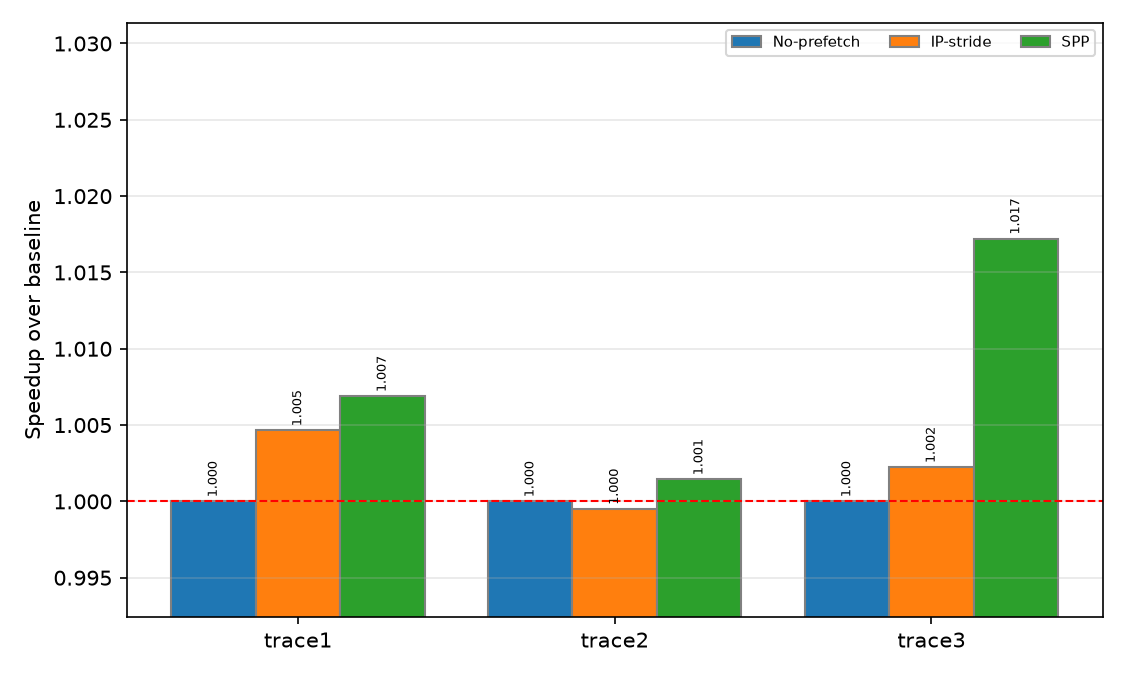
\includegraphics[width=0.8\linewidth]{../plots/task1_speedup.png}
\end{figure}
\begin{figure}[H]
\centering
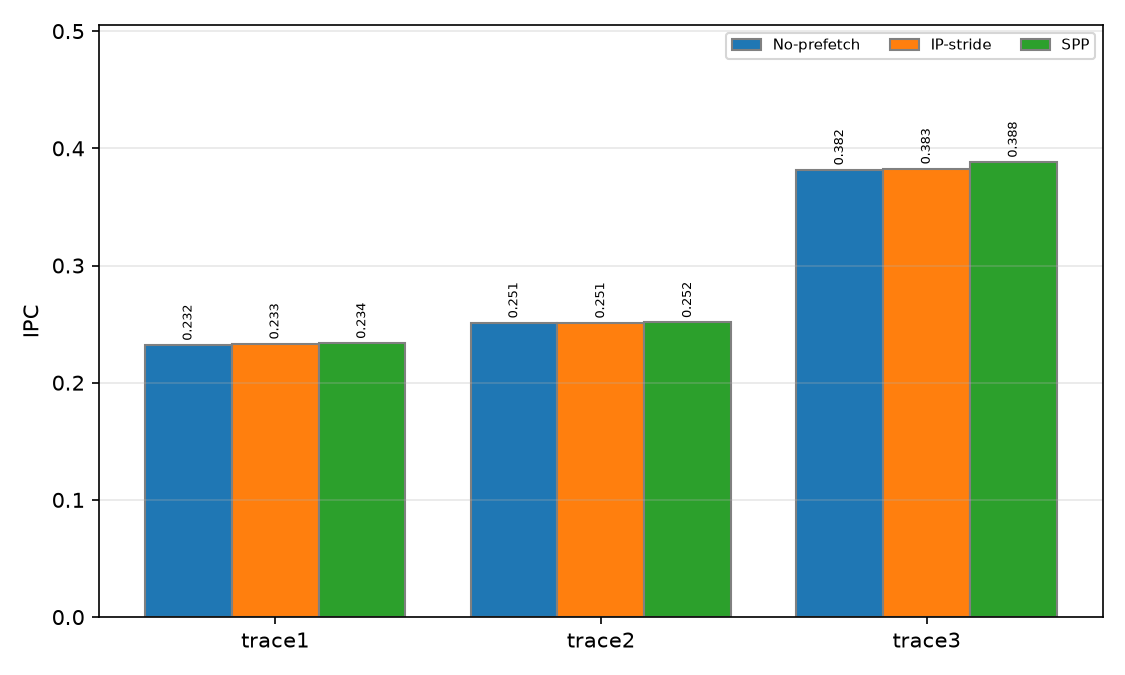
\includegraphics[width=0.8\linewidth]{../plots/task1_ipc.png}
\end{figure}
\begin{figure}[H]
\centering
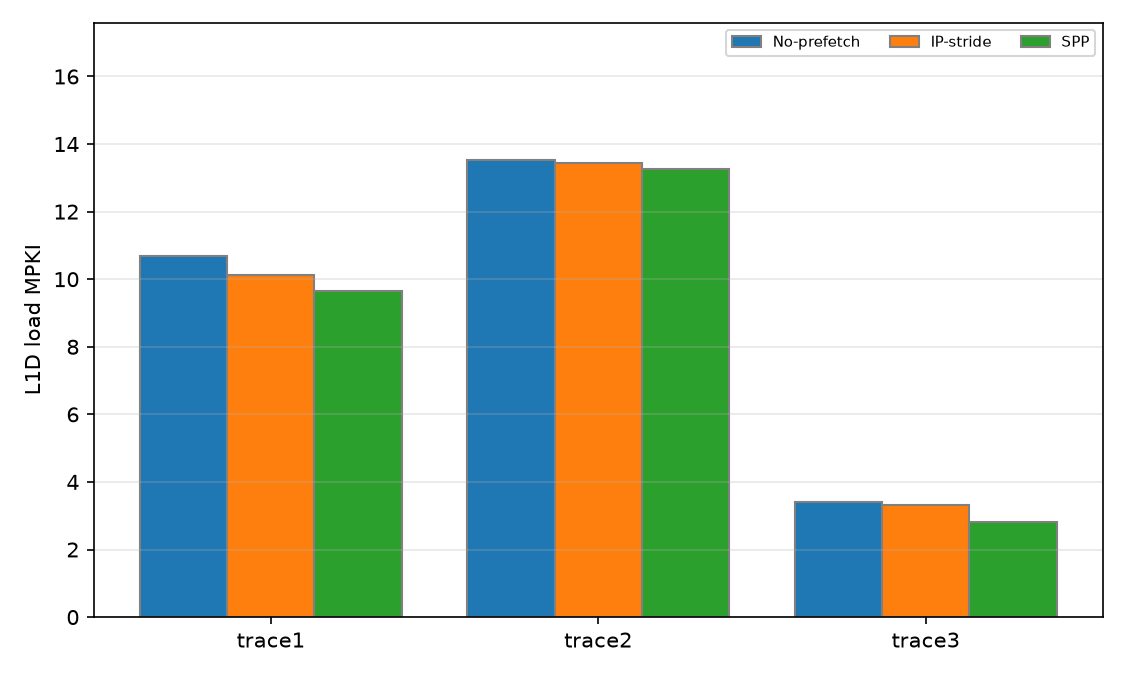
\includegraphics[width=0.8\linewidth]{../plots/task1_l1d_load_mpki.png}
\end{figure}
\begin{figure}[H]
\centering
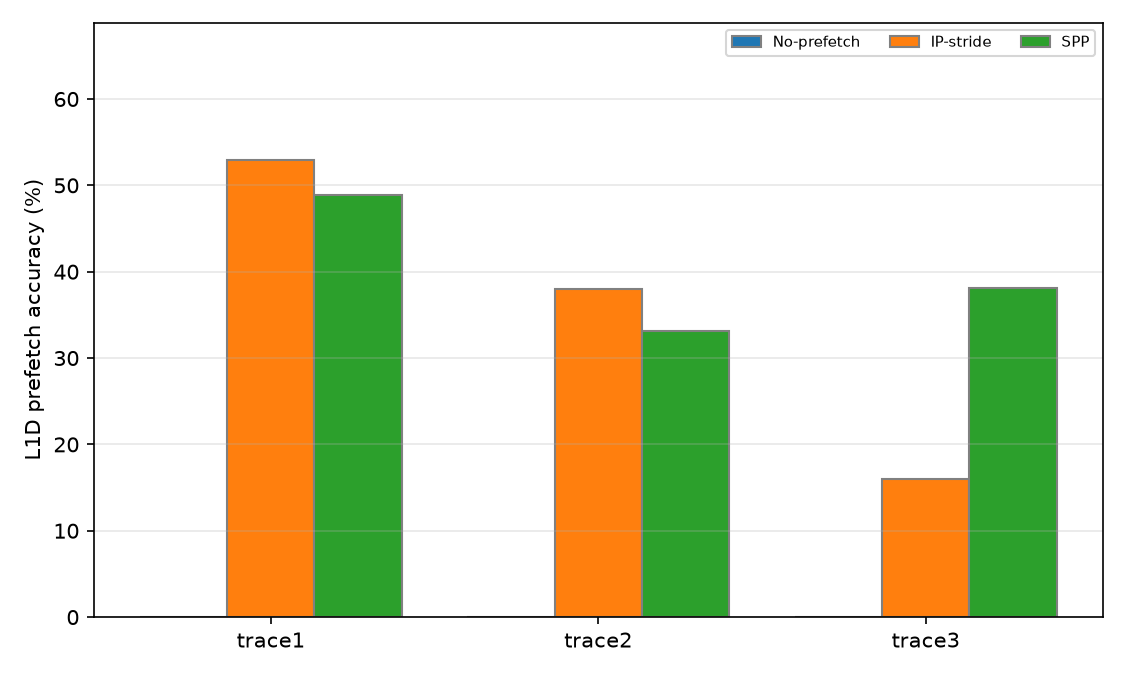
\includegraphics[width=0.8\linewidth]{../plots/task1_l1d_pf_accuracy.png}
\end{figure}
\begin{figure}[H]
\centering
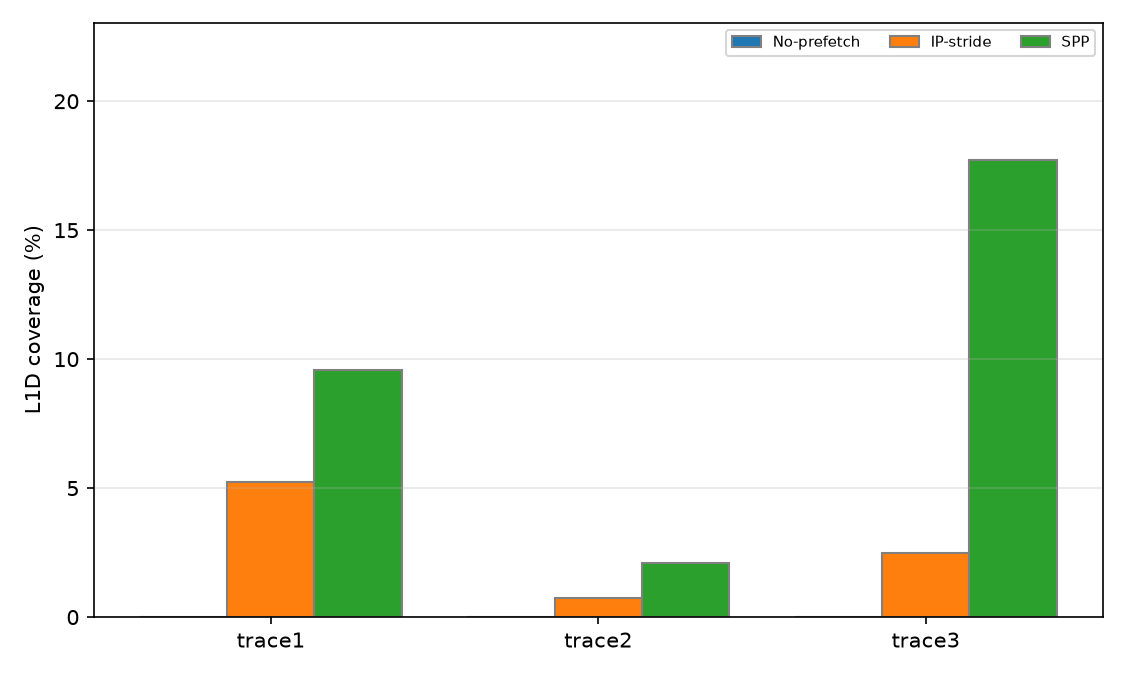
\includegraphics[width=0.8\linewidth]{../plots/task1_l1d_coverage.png}
\end{figure}


\begin{itemize}
\tightlist
\item SPP beats IP-stride on every trace, with 1.8-7x the coverage. Accuracy is a bit lower on trace1/trace2 (49\% vs 53\%, 33\% vs 38\%) and much higher on trace3 (38\% vs 16\%).
\item Both paths fire on the real traces, the non-uniform one issues 50-74\% of the prefetches.
\item The absolute gains are small since even SPP covers only 2-18\% of the L1D misses on these traces.
\end{itemize}

\subsection{Design variants}

Each variant below changes one knob of the final design:


\begin{center}
\begin{minipage}[t]{0.48\linewidth}\centering
\textbf{Speedup}\\[3pt]
\begin{adjustbox}{max width=\linewidth}
\begin{tabular}{@{}lrrrr@{}}
\toprule
\textbf{config} & \textbf{trace1} & \textbf{trace2} & \textbf{trace3} & \textbf{geomean} \\
\midrule
SPP (final) & 1.0069 & 1.0014 & 1.0172 & 1.0085 \\
uniform-only & 1.0064 & 1.0003 & 1.0062 & 1.0043 \\
uniform needs 3 equal strides & 1.0063 & 1.0014 & 1.0163 & 1.0080 \\
fixed degree 4 (no throttle) & 1.0068 & 1.0008 & 1.0169 & 1.0082 \\
degrees 2/4/6/8 & 1.0063 & 1.0009 & 1.0163 & 1.0078 \\
thresholds 40/60/80\% & 1.0073 & 1.0018 & 1.0158 & 1.0083 \\
\bottomrule
\end{tabular}
\end{adjustbox}
\end{minipage}\hfill
\begin{minipage}[t]{0.48\linewidth}\centering
\textbf{L1D prefetch accuracy (\%)}\\[3pt]
\begin{adjustbox}{max width=\linewidth}
\begin{tabular}{@{}lrrr@{}}
\toprule
\textbf{config} & \textbf{trace1} & \textbf{trace2} & \textbf{trace3} \\
\midrule
SPP (final) & 48.8 & 33.1 & 38.1 \\
uniform-only & 54.4 & 37.8 & 27.0 \\
uniform needs 3 equal strides & 49.4 & 33.2 & 41.3 \\
fixed degree 4 (no throttle) & 48.6 & 31.8 & 37.3 \\
degrees 2/4/6/8 & 46.6 & 30.3 & 33.9 \\
thresholds 40/60/80\% & 50.0 & 35.4 & 38.1 \\
\bottomrule
\end{tabular}
\end{adjustbox}
\end{minipage}
\end{center}

\begin{figure}[H]
\centering
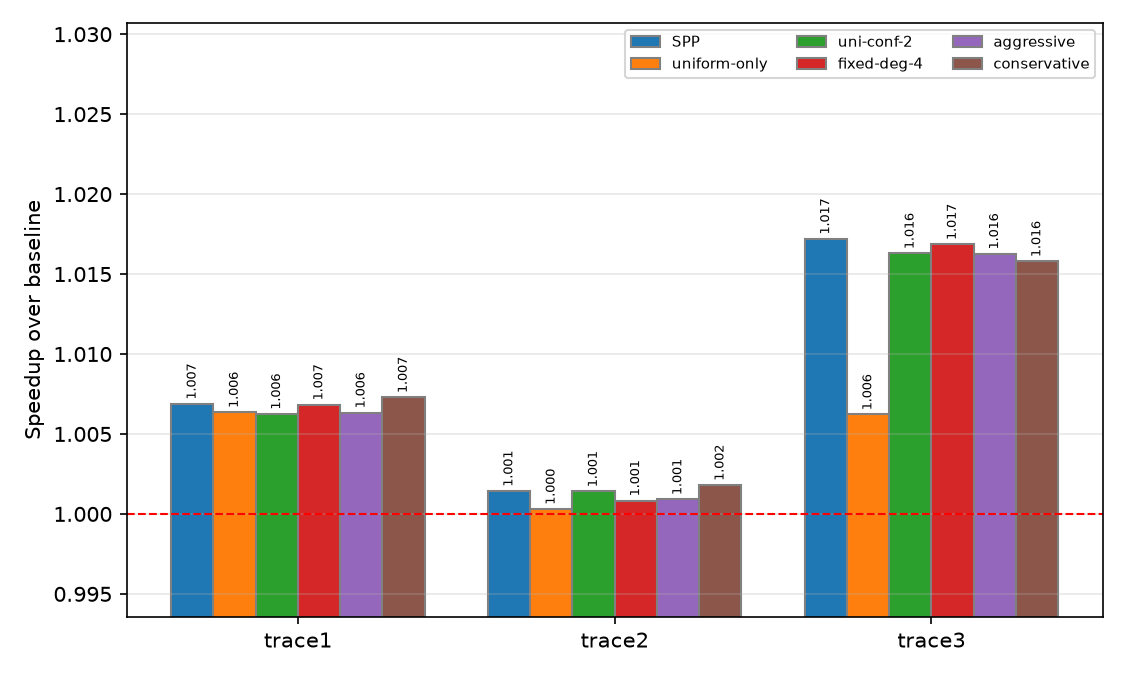
\includegraphics[width=0.8\linewidth]{../plots/task1_variants_speedup.png}
\end{figure}
\begin{figure}[H]
\centering
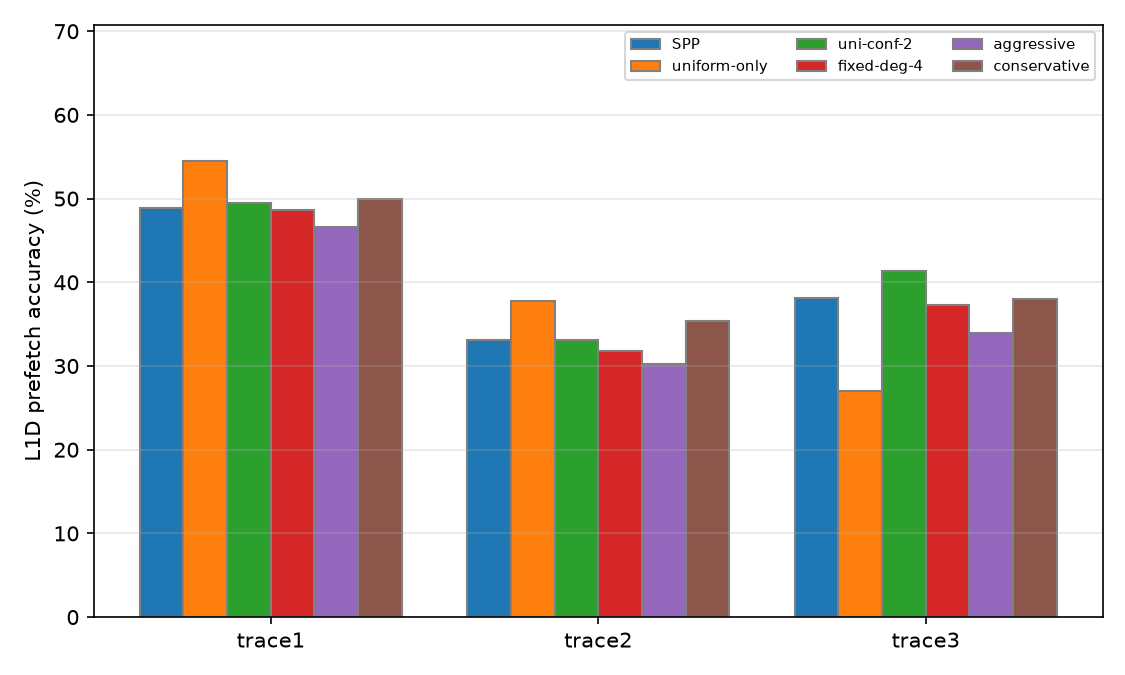
\includegraphics[width=0.8\linewidth]{../plots/task1_variants_l1d_pf_accuracy.png}
\end{figure}


\begin{itemize}
\tightlist
\item Most of the gain comes from the non-uniform path. Without it the geomean halves (1.0043), and trace3 coverage drops from 17.7\% to 7.4\%.
\item Without throttling (fixed degree 4), accuracy drops and speedup is lower on every trace; trace2 loses almost half of its gain (1.0008 vs 1.0014).
\end{itemize}

\subsection{Thresholds and degrees}

\begin{itemize}
\tightlist
\item Thresholds: the throttle splits accuracy into quarters (25/50/75\%). Below 25\% most prefetches just waste bandwidth and L1D space, so SPP issues the minimum. Above 75\% almost all of them get used, so it runs far ahead. Stricter thresholds (40/60/80\%) gave 1-2 points more accuracy and slightly more speedup on trace1/trace2, but lost 0.14\% on trace3 and a bit of geomean (1.0083 vs 1.0085), so we kept the quarters.
\item Degree 1 (not 0) at low accuracy: the throttle measures accuracy only from the prefetches SPP issues, so it has to keep a few going to notice when a phase becomes predictable again.
\item 2 and 4: doubling per range, so each step is a clear change.
\item 6 at the top, not 8: prefetches can't leave the page (64 lines) anyway, and 2/4/6/8 is worse on every trace, with 2-4 points less accuracy, i.e. more pollution for nothing.
\item Degree 4 is the most common on all traces (trace1: 0/148/654/566 windows at degree 1/2/4/6). Degree 1 is rare here, since accuracy almost never falls below 25\%, but it stays as the safety net for bad phases.
\end{itemize}

\subsection{Storage}

The code masks every field to these widths.


\begin{center}
\begin{adjustbox}{max width=\linewidth}
\begin{tabular}{@{}llrr@{}}
\toprule
\textbf{structure} & \textbf{per entry} & \textbf{entries} & \textbf{bits} \\
\midrule
IP table & valid 1, tag 16, last line 16, stride 7, conf 2, signature 12, LRU 6 = 60 & 64 & 3840 \\
pattern table & stride 7, conf 2 = 9 & 1024 & 9216 \\
prefetch filter & line tag 16, valid 1 = 17 (+5-bit pointer) & 32 & 549 \\
accuracy checker & line tag 16, valid 1 = 17 (+7-bit pointer) & 128 & 2183 \\
throttle & issued count 9, useful count 9, degree 3 & 1 & 21 \\
total &  &  & 15809 (1.93 KB) \\
\bottomrule
\end{tabular}
\end{adjustbox}
\end{center}


\clearpage
\section{Task 2: Instruction-conscious L2 replacement}

No prefetchers here, only the L2C policy changes. To give the policy the line type, every call site now passes a new \texttt{isInstruction} argument to \texttt{*\_update\_replacement\_state} (they all share one function-pointer type), filled from the packet's \texttt{instruction} flag. A line counts as code when it's an instruction LOAD/PREFETCH, which is the same rule \texttt{fill\_cache()} uses for \texttt{BLOCK::instruction}.


\subsection{Task 2A: I-RRIP (\texttt{replacement/irrip.l2c\_repl})}

Why favour code at all: an L1I miss that also misses in L2 starves the frontend, the ROB drains and nothing can make progress. A data miss is partly hidden by out-of-order execution. So per line of L2, code is worth more.


\begin{itemize}
\tightlist
\item Insertion (changed): I-RRIP inserts code at RRPV 0 and data at 2 (the SRRIP default). So new code survives two more aging rounds than data, and a burst of data ages out before it can push code out.
\item Promotion (not changed): any hit goes to 0, for both code and data. A hit is direct proof that the line got reused, and demoting data hits would throw that away, which only hurts data-heavy phases and gives the frontend nothing.
\item Eviction (changed): among lines at RRPV 3, I-RRIP evicts data before code. If only code is at 3, it still evicts one of them (no extra aging round), so data never starves and an all-code set behaves like SRRIP.
\item Storage: nothing beyond SRRIP's 2-bit RRPV per line, the 1-bit instruction flag is already in the block.
\end{itemize}

\begin{center}
\begin{minipage}[t]{0.48\linewidth}\centering
\textbf{IPC}\\[3pt]
\begin{adjustbox}{max width=\linewidth}
\begin{tabular}{@{}lrrr@{}}
\toprule
\textbf{config} & \textbf{trace1} & \textbf{trace2} & \textbf{trace3} \\
\midrule
LRU & 0.2322 & 0.2513 & 0.3819 \\
SRRIP & 0.2322 & 0.2518 & 0.3816 \\
I-RRIP & 0.2321 & 0.2564 & 0.3818 \\
\bottomrule
\end{tabular}
\end{adjustbox}
\end{minipage}\hfill
\begin{minipage}[t]{0.48\linewidth}\centering
\textbf{Speedup}\\[3pt]
\begin{adjustbox}{max width=\linewidth}
\begin{tabular}{@{}lrrrr@{}}
\toprule
\textbf{config} & \textbf{trace1} & \textbf{trace2} & \textbf{trace3} & \textbf{geomean} \\
\midrule
LRU & 1.0000 & 1.0000 & 1.0000 & 1.0000 \\
SRRIP & 0.9999 & 1.0022 & 0.9993 & 1.0004 \\
I-RRIP & 0.9995 & 1.0204 & 0.9999 & 1.0065 \\
\bottomrule
\end{tabular}
\end{adjustbox}
\end{minipage}
\end{center}
\medskip
\begin{center}
\begin{minipage}[t]{0.48\linewidth}\centering
\textbf{L2C load MPKI}\\[3pt]
\begin{adjustbox}{max width=\linewidth}
\begin{tabular}{@{}lrrr@{}}
\toprule
\textbf{config} & \textbf{trace1} & \textbf{trace2} & \textbf{trace3} \\
\midrule
LRU & 17.70 & 27.56 & 3.96 \\
SRRIP & 17.62 & 26.01 & 4.04 \\
I-RRIP & 17.72 & 23.00 & 3.94 \\
\bottomrule
\end{tabular}
\end{adjustbox}
\end{minipage}\hfill
\begin{minipage}[t]{0.48\linewidth}\centering
\textbf{L2C instruction load MPKI}\\[3pt]
\begin{adjustbox}{max width=\linewidth}
\begin{tabular}{@{}lrrr@{}}
\toprule
\textbf{config} & \textbf{trace1} & \textbf{trace2} & \textbf{trace3} \\
\midrule
LRU & 10.37 & 18.89 & 1.12 \\
SRRIP & 10.56 & 17.98 & 1.19 \\
I-RRIP & 9.98 & 13.78 & 1.04 \\
\bottomrule
\end{tabular}
\end{adjustbox}
\end{minipage}
\end{center}
\medskip
\begin{center}
\begin{minipage}[t]{0.48\linewidth}\centering
\textbf{L2C data load MPKI}\\[3pt]
\begin{adjustbox}{max width=\linewidth}
\begin{tabular}{@{}lrrr@{}}
\toprule
\textbf{config} & \textbf{trace1} & \textbf{trace2} & \textbf{trace3} \\
\midrule
LRU & 7.33 & 8.67 & 2.84 \\
SRRIP & 7.06 & 8.03 & 2.85 \\
I-RRIP & 7.74 & 9.23 & 2.89 \\
\bottomrule
\end{tabular}
\end{adjustbox}
\end{minipage}
\end{center}

\begin{figure}[H]
\centering
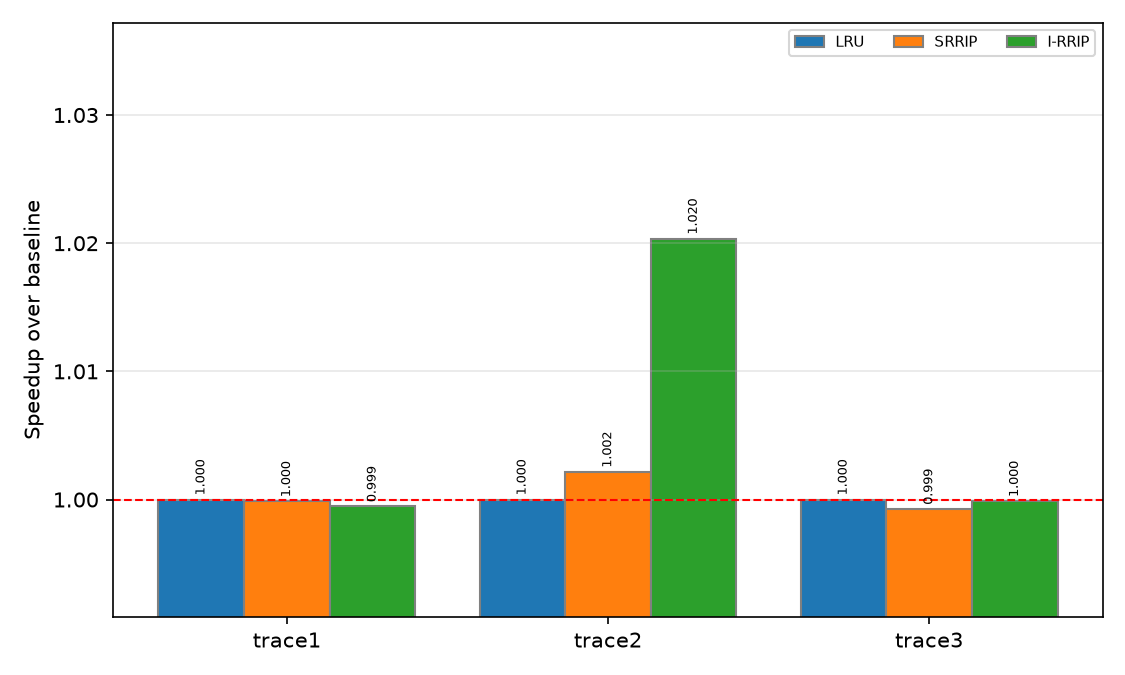
\includegraphics[width=0.8\linewidth]{../plots/task2a_speedup.png}
\end{figure}
\begin{figure}[H]
\centering
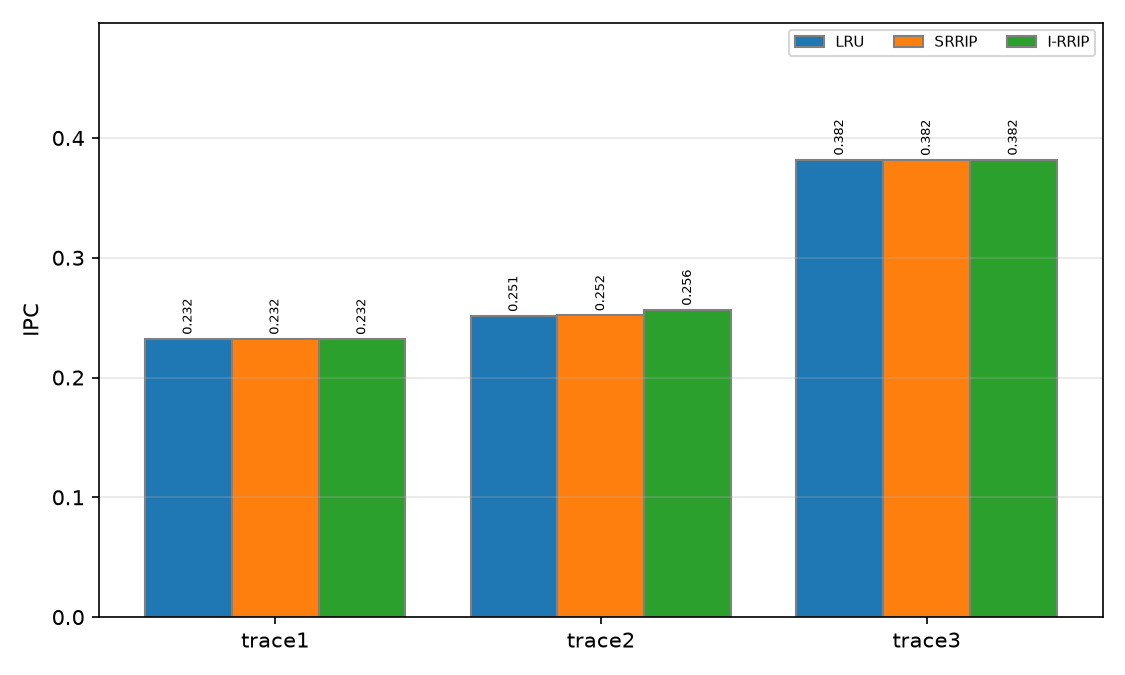
\includegraphics[width=0.8\linewidth]{../plots/task2a_ipc.png}
\end{figure}
\begin{figure}[H]
\centering
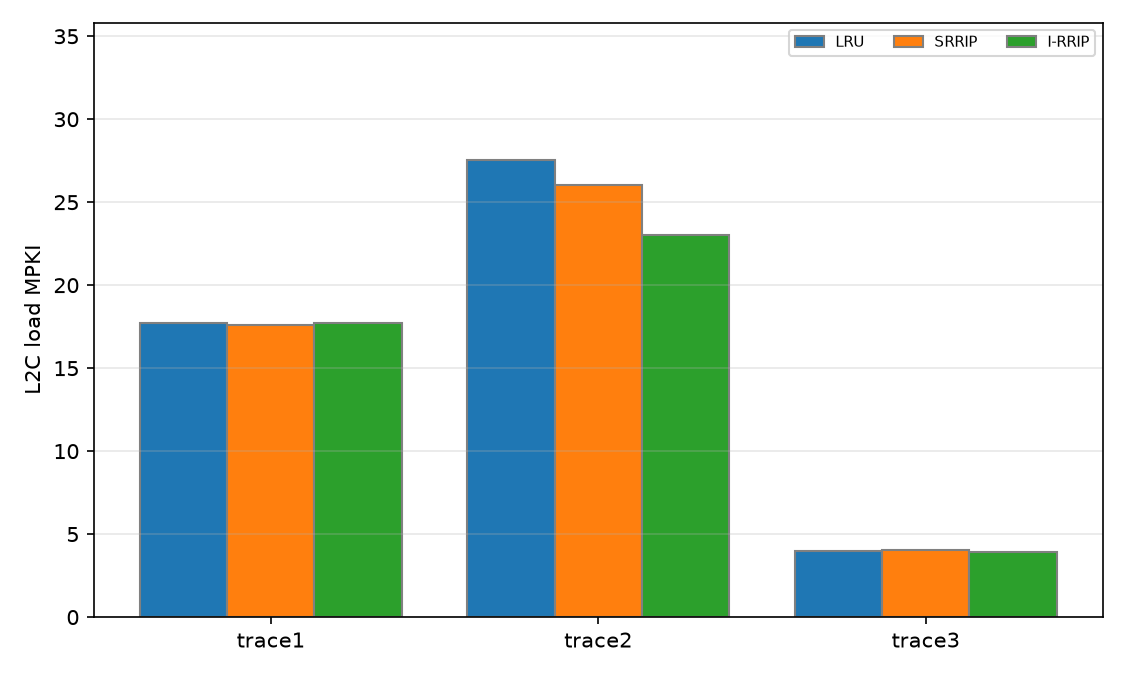
\includegraphics[width=0.8\linewidth]{../plots/task2a_l2c_load_mpki.png}
\end{figure}
\begin{figure}[H]
\centering
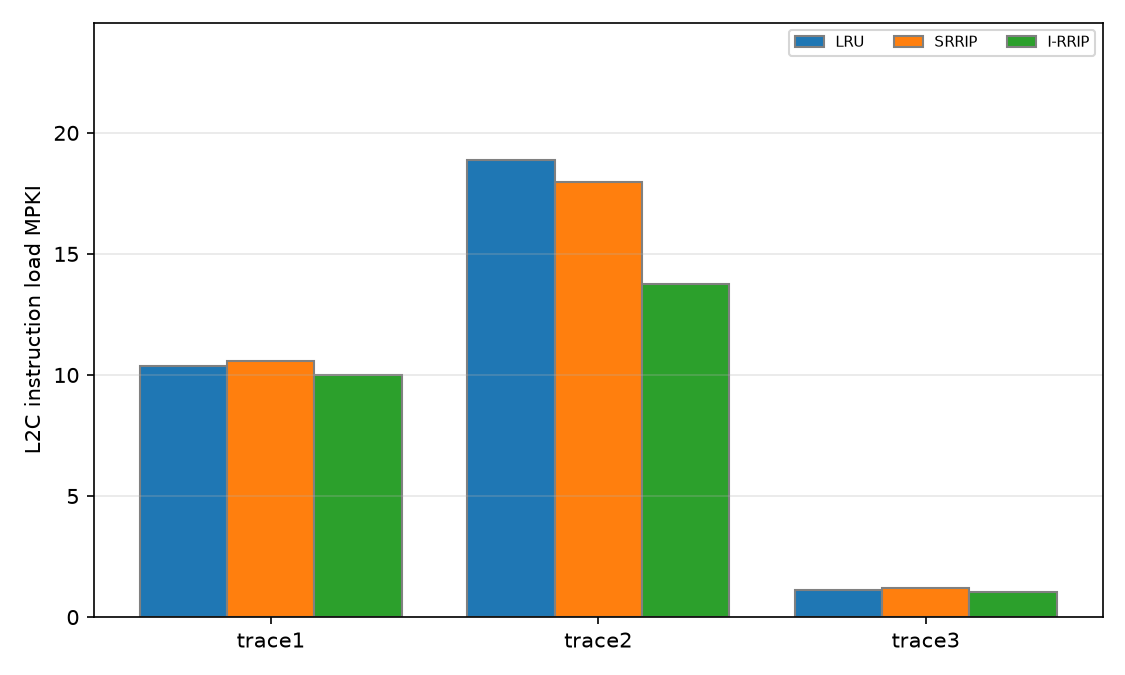
\includegraphics[width=0.8\linewidth]{../plots/task2a_l2c_instr_load_mpki.png}
\end{figure}
\begin{figure}[H]
\centering
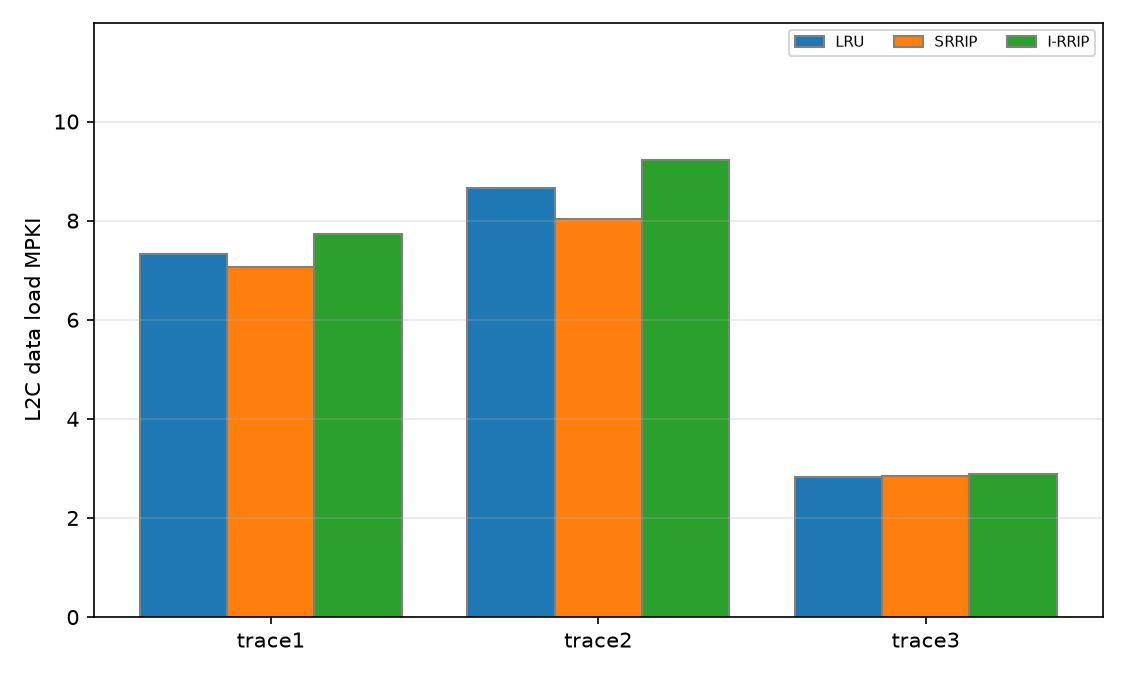
\includegraphics[width=0.8\linewidth]{../plots/task2a_l2c_data_load_mpki.png}
\end{figure}


\begin{itemize}
\tightlist
\item I-RRIP cuts L2 instruction MPKI on every trace (-27\% on trace2), for a smaller rise in data MPKI.
\item Only trace2 turns this into IPC (+2.0\%). On trace1/trace3 most L2 misses also miss the LLC, and those DRAM-bound misses are mostly data, which an instruction-favouring L2 can't remove.
\end{itemize}

\subsubsection{Why this combination is the best}

Each alternative below changes one knob in the same file:


\begin{center}
\begin{minipage}[t]{0.48\linewidth}\centering
\textbf{Speedup}\\[3pt]
\begin{adjustbox}{max width=\linewidth}
\begin{tabular}{@{}lrrrr@{}}
\toprule
\textbf{config} & \textbf{trace1} & \textbf{trace2} & \textbf{trace3} & \textbf{geomean} \\
\midrule
I-RRIP (code 0, data 2, data-first) & 0.9995 & 1.0204 & 0.9999 & 1.0065 \\
code inserted at 1 & 0.9998 & 1.0193 & 0.9996 & 1.0062 \\
no data-first eviction & 0.9998 & 1.0132 & 0.9999 & 1.0043 \\
data inserted at 3 & 0.9960 & 1.0307 & 0.9999 & 1.0088 \\
\bottomrule
\end{tabular}
\end{adjustbox}
\end{minipage}\hfill
\begin{minipage}[t]{0.48\linewidth}\centering
\textbf{L2C instruction load MPKI}\\[3pt]
\begin{adjustbox}{max width=\linewidth}
\begin{tabular}{@{}lrrr@{}}
\toprule
\textbf{config} & \textbf{trace1} & \textbf{trace2} & \textbf{trace3} \\
\midrule
I-RRIP (code 0, data 2, data-first) & 9.98 & 13.78 & 1.04 \\
code inserted at 1 & 10.05 & 13.96 & 1.07 \\
no data-first eviction & 10.14 & 15.71 & 1.08 \\
data inserted at 3 & 9.39 & 9.51 & 0.85 \\
\bottomrule
\end{tabular}
\end{adjustbox}
\end{minipage}
\end{center}

\begin{figure}[H]
\centering
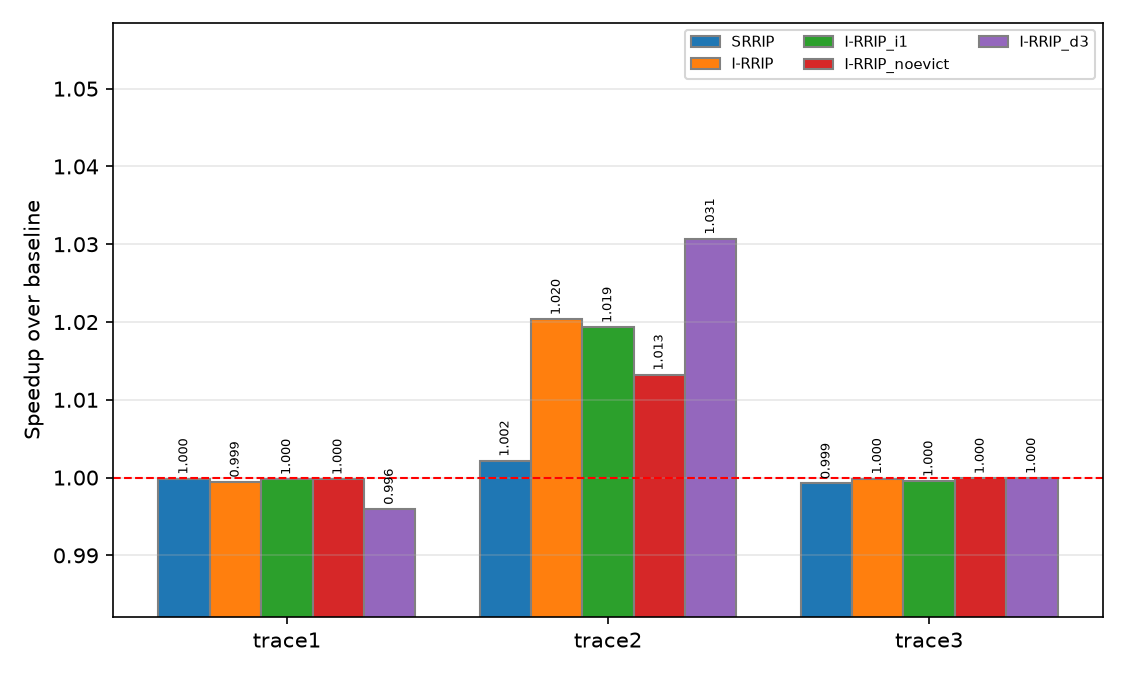
\includegraphics[width=0.8\linewidth]{../plots/task2a_variants_speedup.png}
\end{figure}
\begin{figure}[H]
\centering
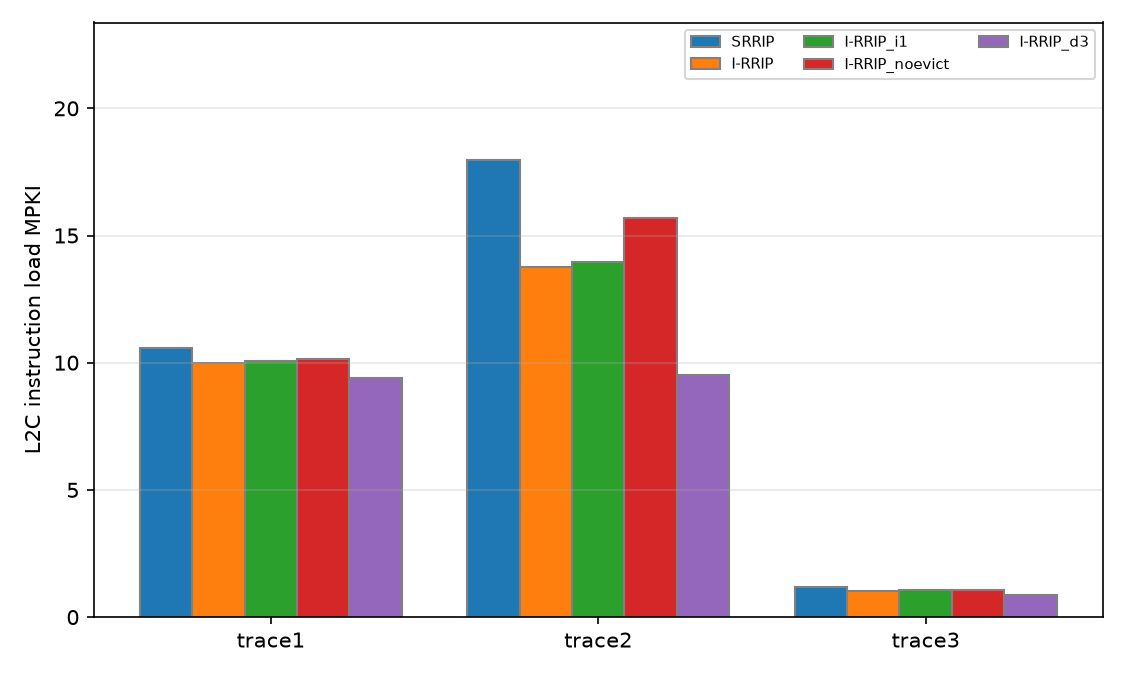
\includegraphics[width=0.8\linewidth]{../plots/task2a_variants_l2c_instr_load_mpki.png}
\end{figure}


\begin{itemize}
\tightlist
\item Data-first eviction matters the most: without it trace2 keeps 14\% more instruction misses and loses a third of its speedup. Insertion alone isn't enough, since everything ages together and code still reaches RRPV 3 and competes with data there.
\item Code at 0 vs 1 is almost the same, 0 is slightly better on trace2.
\item Data at 3 protects code harder (best trace2, +3.1\%), but costs trace1 0.4\%. So blindly favouring code hurts data-heavy workloads, which is why static I-RRIP keeps data at 2, and only the dynamic policy, which can turn it off, uses 3.
\end{itemize}

\subsection{Task 2B: Dynamic I-RRIP (\texttt{replacement/dyn\_irrip.l2c\_repl})}

\subsubsection{Leader sets}

\begin{itemize}
\tightlist
\item The policy splits the 1024 sets into 32 groups of 32. In each group one set always runs SRRIP (high 5 index bits == low 5 bits) and one always runs I-RRIP (high 5 bits == \textasciitilde{}low 5 bits). So 64 leaders, spread over the whole cache.
\item 1 in 32 sets per policy gives enough samples to follow a phase change within a few thousand accesses, while only 6\% of the cache is stuck on a policy that might be wrong. It's also the usual DIP choice for 1024 sets.
\end{itemize}

\subsubsection{Decision logic}

\begin{itemize}
\tightlist
\item The SRRIP leaders count instruction / total accesses and misses, ignoring writebacks (they never stall the core), and the policy computes the ratio from the hint:

\begin{verbatim}
(instr accesses + instr misses) / (total accesses + total misses)
\end{verbatim}
\end{itemize}
  with integer math (\texttt{100 * num $>$ pct * den}). The counters halve every 16K leader accesses, so old phases fade out.

\begin{itemize}
\tightlist
\item Sampling happens on SRRIP leaders on purpose, not I-RRIP ones: under I-RRIP the instruction misses would shrink and the ratio would talk itself out of I-RRIP mode.
\item Our extension, a miss duel: a 10-bit PSEL goes up on every demand miss in an SRRIP leader and down on every one in an I-RRIP leader. Followers use I-RRIP only if ratio $>$ 25\% \textbf{and} PSEL $\geq$ 512. The ratio says whether code is a big share of the traffic, the duel says whether favouring it is actually winning.
\item Since the duel vetoes I-RRIP where it's losing, I-RRIP mode inserts data at 3 (the aggressive variant from 2A).
\item Storage: SRRIP's RRPVs + four 14-bit counters + a 10-bit PSEL = 66 bits.
\end{itemize}

\subsubsection{Threshold sensitivity (ratio only, no duel, data at 2)}

\begin{center}
\begin{minipage}[t]{0.48\linewidth}\centering
\textbf{Speedup}\\[3pt]
\begin{adjustbox}{max width=\linewidth}
\begin{tabular}{@{}lrrrr@{}}
\toprule
\textbf{threshold} & \textbf{trace1} & \textbf{trace2} & \textbf{trace3} & \textbf{geomean} \\
\midrule
10\% & 0.9993 & 1.0197 & 0.9998 & 1.0062 \\
25\% & 0.9996 & 1.0196 & 0.9997 & 1.0062 \\
40\% & 0.9996 & 1.0176 & 0.9993 & 1.0055 \\
55\% & 0.9999 & 1.0112 & 0.9993 & 1.0034 \\
70\% & 0.9999 & 1.0022 & 0.9993 & 1.0004 \\
\bottomrule
\end{tabular}
\end{adjustbox}
\end{minipage}\hfill
\begin{minipage}[t]{0.48\linewidth}\centering
\textbf{L2C instruction load MPKI}\\[3pt]
\begin{adjustbox}{max width=\linewidth}
\begin{tabular}{@{}lrrr@{}}
\toprule
\textbf{threshold} & \textbf{trace1} & \textbf{trace2} & \textbf{trace3} \\
\midrule
10\% & 10.00 & 13.92 & 1.05 \\
25\% & 9.99 & 13.93 & 1.05 \\
40\% & 9.99 & 14.37 & 1.12 \\
55\% & 10.56 & 15.68 & 1.19 \\
70\% & 10.56 & 17.98 & 1.19 \\
\bottomrule
\end{tabular}
\end{adjustbox}
\end{minipage}
\end{center}

\begin{figure}[H]
\centering
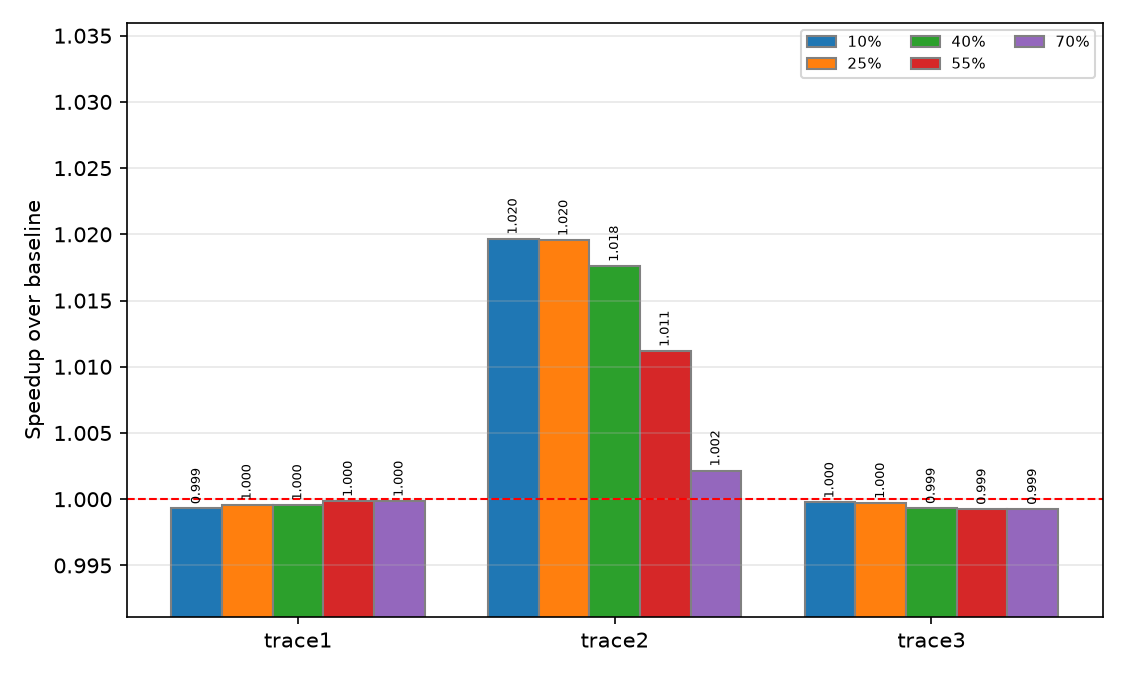
\includegraphics[width=0.8\linewidth]{../plots/task2b_threshold_speedup.png}
\end{figure}
\begin{figure}[H]
\centering
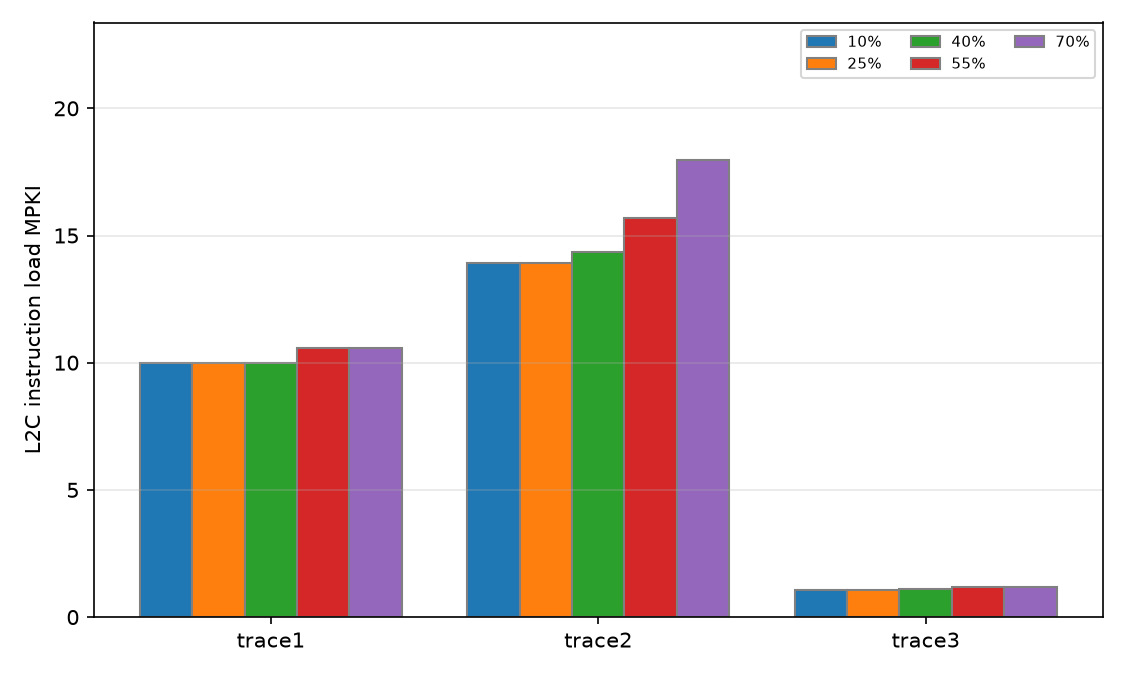
\includegraphics[width=0.8\linewidth]{../plots/task2b_threshold_l2c_instr_load_mpki.png}
\end{figure}


\begin{itemize}
\tightlist
\item 10-25\% keep I-RRIP on almost always (90-100\% of follower fills) and match static I-RRIP. 70\% never turns it on and matches SRRIP.
\item We picked 25\%: as good as 10\% on trace2, slightly better on trace1.
\item The sweep also shows the ratio's limit: trace1 is code-heavy (it stays in I-RRIP mode up to 40\%), yet favouring code isn't helping it. That's why we added the duel.
\end{itemize}

\subsubsection{Final policy}

\begin{center}
\begin{minipage}[t]{0.48\linewidth}\centering
\textbf{IPC}\\[3pt]
\begin{adjustbox}{max width=\linewidth}
\begin{tabular}{@{}lrrr@{}}
\toprule
\textbf{config} & \textbf{trace1} & \textbf{trace2} & \textbf{trace3} \\
\midrule
LRU & 0.2322 & 0.2513 & 0.3819 \\
SRRIP & 0.2322 & 0.2518 & 0.3816 \\
I-RRIP & 0.2321 & 0.2564 & 0.3818 \\
Dyn (ratio only) & 0.2322 & 0.2562 & 0.3817 \\
Dyn-I-RRIP (final) & 0.2321 & 0.2586 & 0.3815 \\
\bottomrule
\end{tabular}
\end{adjustbox}
\end{minipage}\hfill
\begin{minipage}[t]{0.48\linewidth}\centering
\textbf{Speedup}\\[3pt]
\begin{adjustbox}{max width=\linewidth}
\begin{tabular}{@{}lrrrr@{}}
\toprule
\textbf{config} & \textbf{trace1} & \textbf{trace2} & \textbf{trace3} & \textbf{geomean} \\
\midrule
LRU & 1.0000 & 1.0000 & 1.0000 & 1.0000 \\
SRRIP & 0.9999 & 1.0022 & 0.9993 & 1.0004 \\
I-RRIP & 0.9995 & 1.0204 & 0.9999 & 1.0065 \\
Dyn (ratio only) & 0.9996 & 1.0196 & 0.9997 & 1.0062 \\
Dyn-I-RRIP (final) & 0.9994 & 1.0290 & 0.9992 & 1.0091 \\
\bottomrule
\end{tabular}
\end{adjustbox}
\end{minipage}
\end{center}
\medskip
\begin{center}
\begin{minipage}[t]{0.48\linewidth}\centering
\textbf{L2C load MPKI}\\[3pt]
\begin{adjustbox}{max width=\linewidth}
\begin{tabular}{@{}lrrr@{}}
\toprule
\textbf{config} & \textbf{trace1} & \textbf{trace2} & \textbf{trace3} \\
\midrule
LRU & 17.70 & 27.56 & 3.96 \\
SRRIP & 17.62 & 26.01 & 4.04 \\
I-RRIP & 17.72 & 23.00 & 3.94 \\
Dyn (ratio only) & 17.70 & 23.14 & 3.94 \\
Dyn-I-RRIP (final) & 17.65 & 20.59 & 4.04 \\
\bottomrule
\end{tabular}
\end{adjustbox}
\end{minipage}\hfill
\begin{minipage}[t]{0.48\linewidth}\centering
\textbf{L2C instruction load MPKI}\\[3pt]
\begin{adjustbox}{max width=\linewidth}
\begin{tabular}{@{}lrrr@{}}
\toprule
\textbf{config} & \textbf{trace1} & \textbf{trace2} & \textbf{trace3} \\
\midrule
LRU & 10.37 & 18.89 & 1.12 \\
SRRIP & 10.56 & 17.98 & 1.19 \\
I-RRIP & 9.98 & 13.78 & 1.04 \\
Dyn (ratio only) & 9.99 & 13.93 & 1.05 \\
Dyn-I-RRIP (final) & 10.52 & 10.02 & 1.18 \\
\bottomrule
\end{tabular}
\end{adjustbox}
\end{minipage}
\end{center}
\medskip
\begin{center}
\begin{minipage}[t]{0.48\linewidth}\centering
\textbf{L2C data load MPKI}\\[3pt]
\begin{adjustbox}{max width=\linewidth}
\begin{tabular}{@{}lrrr@{}}
\toprule
\textbf{config} & \textbf{trace1} & \textbf{trace2} & \textbf{trace3} \\
\midrule
LRU & 7.33 & 8.67 & 2.84 \\
SRRIP & 7.06 & 8.03 & 2.85 \\
I-RRIP & 7.74 & 9.23 & 2.89 \\
Dyn (ratio only) & 7.71 & 9.21 & 2.90 \\
Dyn-I-RRIP (final) & 7.13 & 10.57 & 2.86 \\
\bottomrule
\end{tabular}
\end{adjustbox}
\end{minipage}
\end{center}

\begin{figure}[H]
\centering
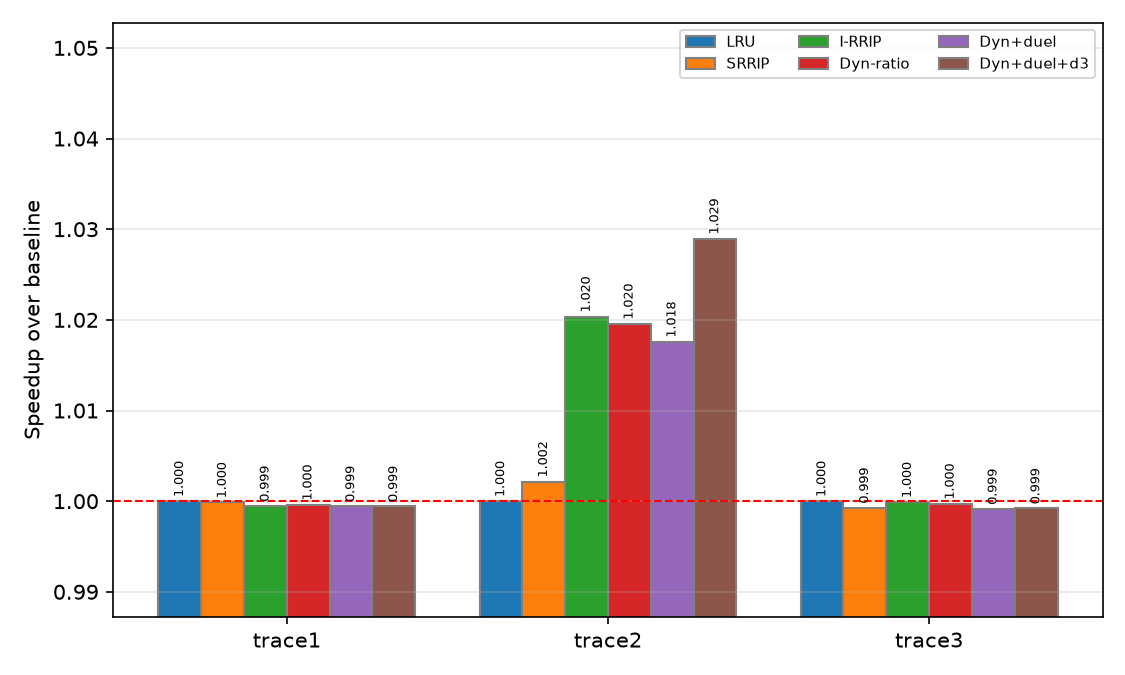
\includegraphics[width=0.8\linewidth]{../plots/task2b_speedup.png}
\end{figure}
\begin{figure}[H]
\centering
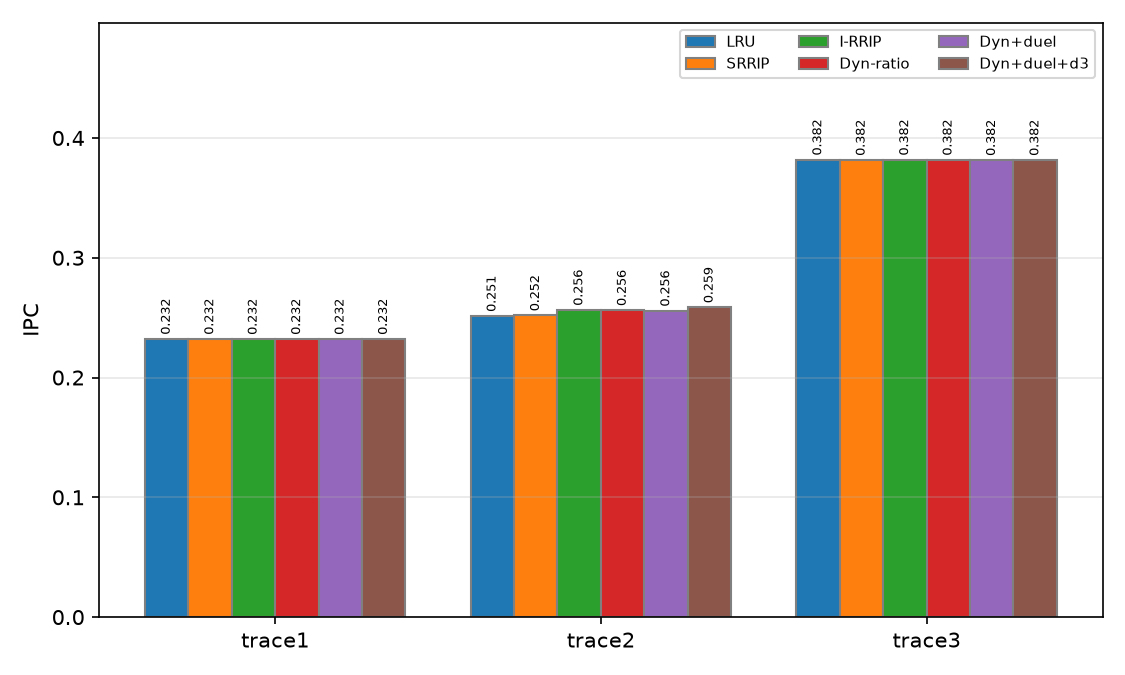
\includegraphics[width=0.8\linewidth]{../plots/task2b_ipc.png}
\end{figure}
\begin{figure}[H]
\centering
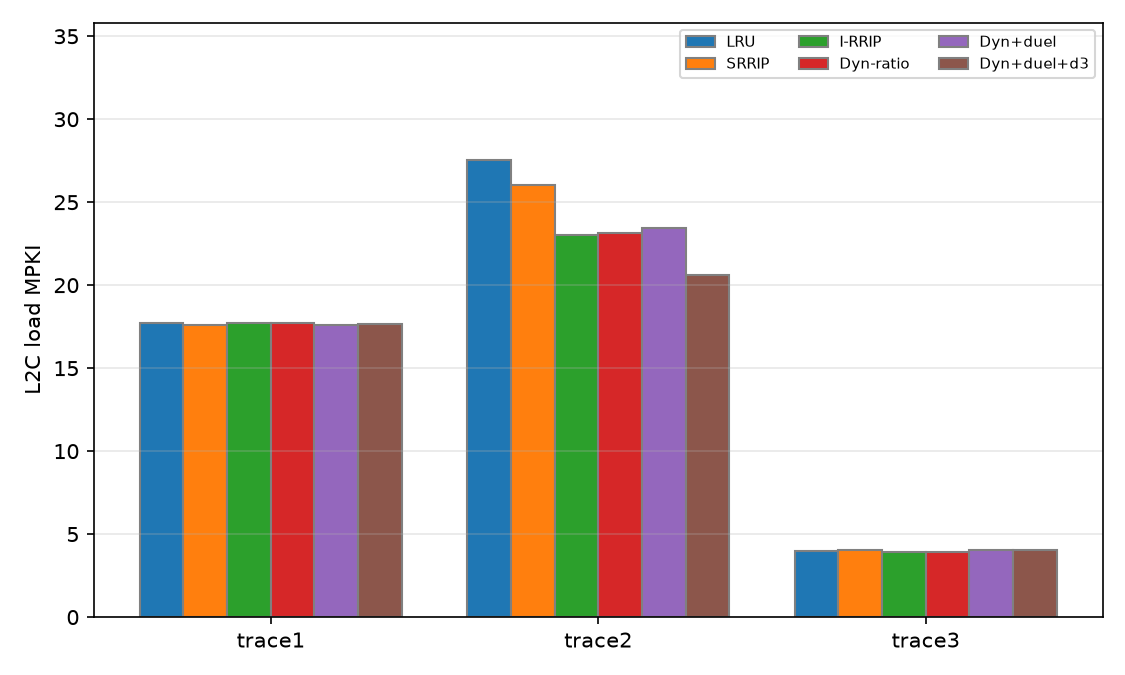
\includegraphics[width=0.8\linewidth]{../plots/task2b_l2c_load_mpki.png}
\end{figure}
\begin{figure}[H]
\centering
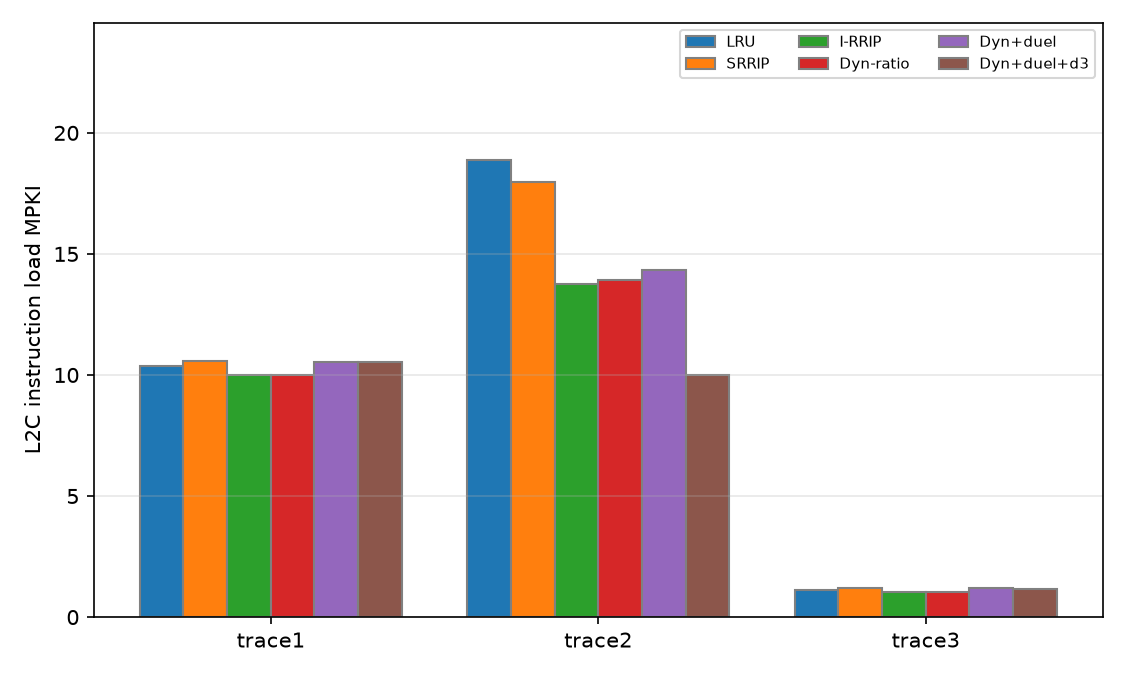
\includegraphics[width=0.8\linewidth]{../plots/task2b_l2c_instr_load_mpki.png}
\end{figure}
\begin{figure}[H]
\centering
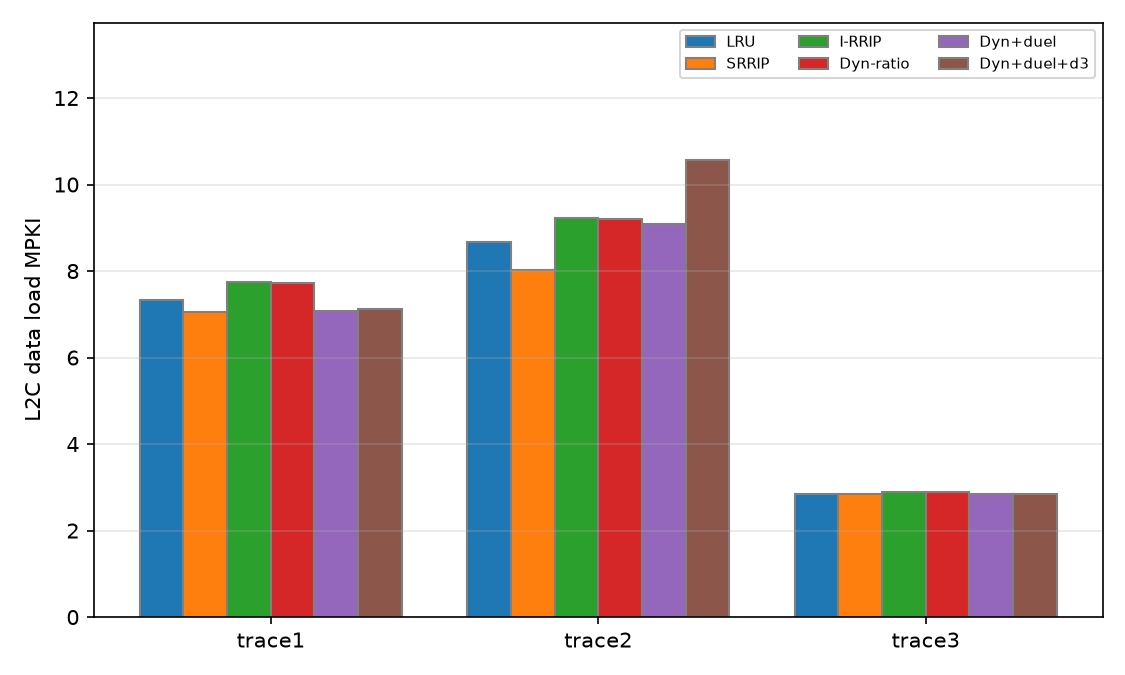
\includegraphics[width=0.8\linewidth]{../plots/task2b_l2c_data_load_mpki.png}
\end{figure}


\begin{itemize}
\tightlist
\item The duel turns I-RRIP off for all of trace1 (0\% of follower fills) and most of trace3 (9\%), and keeping it on for trace2 (56\%, PSEL ends at 931/1023).
\item So we're getting the aggressive variant's trace2 gain (+2.9\%, L2 MPKI 27.6 $\rightarrow$ 20.6) without its trace1 loss, and the best geomean (1.0091).
\item The 0.06-0.08\% left vs LRU on trace1/trace3 is just SRRIP vs LRU, which the followers fall back to there.
\end{itemize}
\clearpage
\section{Task 3: SPP + prefetch-aware Dynamic I-RRIP}

Here SPP (Task 1) runs at the L1D and Dynamic I-RRIP (Task 2B) at the L2C, and the L2C policy becomes prefetch-aware (\texttt{PF\_AWARE=1} in \texttt{replacement/dyn\_irrip.l2c\_repl}).


\subsection{Handling prefetch packets}

Data prefetches reaching the L2C come from SPP (type \texttt{PREFETCH}, not an instruction). They're speculative: nobody has asked for the line yet, and most of them also go into the L1D, so the L2C copy only matters if the L1D drops it before it's used. So until a demand access proves a prefetched line useful, it shouldn't push out code or demand data:


\begin{itemize}
\tightlist
\item Insertion: the policy inserts prefetch fills at RRPV 3 in every set and mode. So bad prefetches evict each other first (SPP is only 32-49\% accurate here).
\item Promotion: a prefetch hitting a line doesn't promote it, only demand hits do. Getting prefetched again says nothing about demand reuse. A demand hit on a prefetched line promotes it to 0 like any other line, so the cache still keeps useful prefetches.
\item Sampling: the ratio counters and PSEL ignore prefetches. Otherwise a prefetch-heavy phase could dilute the instruction share and flip the followers out of I-RRIP for traffic that never stalls the core.
\item No extra storage. Without an L1D prefetcher nothing changes, so the Task 2 numbers still hold.
\end{itemize}

\subsection{Results}

Configs: SPP+Dyn-I-RRIP is the final 2B policy with \texttt{PF\_AWARE=0}, SPP+PF-aware is the final policy, and -pf2 inserts prefetches at 2 instead of 3.


\begin{center}
\begin{minipage}[t]{0.48\linewidth}\centering
\textbf{IPC}\\[3pt]
\begin{adjustbox}{max width=\linewidth}
\begin{tabular}{@{}lrrr@{}}
\toprule
\textbf{config} & \textbf{trace1} & \textbf{trace2} & \textbf{trace3} \\
\midrule
LRU & 0.2322 & 0.2513 & 0.3819 \\
Dyn-I-RRIP & 0.2321 & 0.2586 & 0.3815 \\
SPP+LRU & 0.2338 & 0.2517 & 0.3884 \\
SPP+Dyn-I-RRIP & 0.2338 & 0.2593 & 0.3879 \\
SPP+PF-aware & 0.2339 & 0.2592 & 0.3879 \\
SPP+PF-aware-pf2 & 0.2339 & 0.2588 & 0.3879 \\
\bottomrule
\end{tabular}
\end{adjustbox}
\end{minipage}\hfill
\begin{minipage}[t]{0.48\linewidth}\centering
\textbf{Speedup}\\[3pt]
\begin{adjustbox}{max width=\linewidth}
\begin{tabular}{@{}lrrrr@{}}
\toprule
\textbf{config} & \textbf{trace1} & \textbf{trace2} & \textbf{trace3} & \textbf{geomean} \\
\midrule
LRU & 1.0000 & 1.0000 & 1.0000 & 1.0000 \\
Dyn-I-RRIP & 0.9994 & 1.0290 & 0.9992 & 1.0091 \\
SPP+LRU & 1.0069 & 1.0014 & 1.0172 & 1.0085 \\
SPP+Dyn-I-RRIP & 1.0068 & 1.0318 & 1.0157 & 1.0181 \\
SPP+PF-aware & 1.0073 & 1.0315 & 1.0159 & 1.0182 \\
SPP+PF-aware-pf2 & 1.0071 & 1.0299 & 1.0157 & 1.0175 \\
\bottomrule
\end{tabular}
\end{adjustbox}
\end{minipage}
\end{center}
\medskip
\begin{center}
\begin{minipage}[t]{0.48\linewidth}\centering
\textbf{L1D load MPKI}\\[3pt]
\begin{adjustbox}{max width=\linewidth}
\begin{tabular}{@{}lrrr@{}}
\toprule
\textbf{config} & \textbf{trace1} & \textbf{trace2} & \textbf{trace3} \\
\midrule
LRU & 10.68 & 13.54 & 3.40 \\
SPP+LRU & 9.66 & 13.25 & 2.80 \\
SPP+Dyn-I-RRIP & 9.65 & 13.28 & 2.82 \\
SPP+PF-aware & 9.65 & 13.27 & 2.82 \\
SPP+PF-aware-pf2 & 9.65 & 13.28 & 2.82 \\
\bottomrule
\end{tabular}
\end{adjustbox}
\end{minipage}\hfill
\begin{minipage}[t]{0.48\linewidth}\centering
\textbf{L1D prefetch accuracy (\%)}\\[3pt]
\begin{adjustbox}{max width=\linewidth}
\begin{tabular}{@{}lrrr@{}}
\toprule
\textbf{config} & \textbf{trace1} & \textbf{trace2} & \textbf{trace3} \\
\midrule
SPP+LRU & 48.8 & 33.1 & 38.1 \\
SPP+Dyn-I-RRIP & 48.9 & 32.3 & 37.4 \\
SPP+PF-aware & 49.1 & 32.3 & 37.3 \\
SPP+PF-aware-pf2 & 49.1 & 32.3 & 37.4 \\
\bottomrule
\end{tabular}
\end{adjustbox}
\end{minipage}
\end{center}
\medskip
\begin{center}
\begin{minipage}[t]{0.48\linewidth}\centering
\textbf{L1D coverage (\%)}\\[3pt]
\begin{adjustbox}{max width=\linewidth}
\begin{tabular}{@{}lrrr@{}}
\toprule
\textbf{config} & \textbf{trace1} & \textbf{trace2} & \textbf{trace3} \\
\midrule
SPP+LRU & 9.57 & 2.08 & 17.73 \\
SPP+Dyn-I-RRIP & 9.61 & 1.92 & 17.21 \\
SPP+PF-aware & 9.61 & 1.93 & 17.06 \\
SPP+PF-aware-pf2 & 9.60 & 1.91 & 17.26 \\
\bottomrule
\end{tabular}
\end{adjustbox}
\end{minipage}\hfill
\begin{minipage}[t]{0.48\linewidth}\centering
\textbf{L2C load MPKI}\\[3pt]
\begin{adjustbox}{max width=\linewidth}
\begin{tabular}{@{}lrrr@{}}
\toprule
\textbf{config} & \textbf{trace1} & \textbf{trace2} & \textbf{trace3} \\
\midrule
LRU & 17.70 & 27.56 & 3.96 \\
Dyn-I-RRIP & 17.65 & 20.59 & 4.04 \\
SPP+LRU & 16.86 & 27.78 & 3.24 \\
SPP+Dyn-I-RRIP & 16.84 & 20.52 & 3.31 \\
SPP+PF-aware & 16.73 & 20.48 & 3.29 \\
SPP+PF-aware-pf2 & 16.79 & 20.84 & 3.31 \\
\bottomrule
\end{tabular}
\end{adjustbox}
\end{minipage}
\end{center}
\medskip
\begin{center}
\begin{minipage}[t]{0.48\linewidth}\centering
\textbf{L2C instruction load MPKI}\\[3pt]
\begin{adjustbox}{max width=\linewidth}
\begin{tabular}{@{}lrrr@{}}
\toprule
\textbf{config} & \textbf{trace1} & \textbf{trace2} & \textbf{trace3} \\
\midrule
LRU & 10.37 & 18.89 & 1.12 \\
Dyn-I-RRIP & 10.52 & 10.02 & 1.18 \\
SPP+LRU & 10.41 & 19.36 & 1.16 \\
SPP+Dyn-I-RRIP & 10.57 & 10.00 & 1.20 \\
SPP+PF-aware & 10.49 & 9.96 & 1.18 \\
SPP+PF-aware-pf2 & 10.54 & 10.44 & 1.20 \\
\bottomrule
\end{tabular}
\end{adjustbox}
\end{minipage}\hfill
\begin{minipage}[t]{0.48\linewidth}\centering
\textbf{L2C data load MPKI}\\[3pt]
\begin{adjustbox}{max width=\linewidth}
\begin{tabular}{@{}lrrr@{}}
\toprule
\textbf{config} & \textbf{trace1} & \textbf{trace2} & \textbf{trace3} \\
\midrule
LRU & 7.33 & 8.67 & 2.84 \\
Dyn-I-RRIP & 7.13 & 10.57 & 2.86 \\
SPP+LRU & 6.45 & 8.42 & 2.08 \\
SPP+Dyn-I-RRIP & 6.27 & 10.52 & 2.12 \\
SPP+PF-aware & 6.24 & 10.52 & 2.11 \\
SPP+PF-aware-pf2 & 6.25 & 10.40 & 2.12 \\
\bottomrule
\end{tabular}
\end{adjustbox}
\end{minipage}
\end{center}

\begin{figure}[H]
\centering
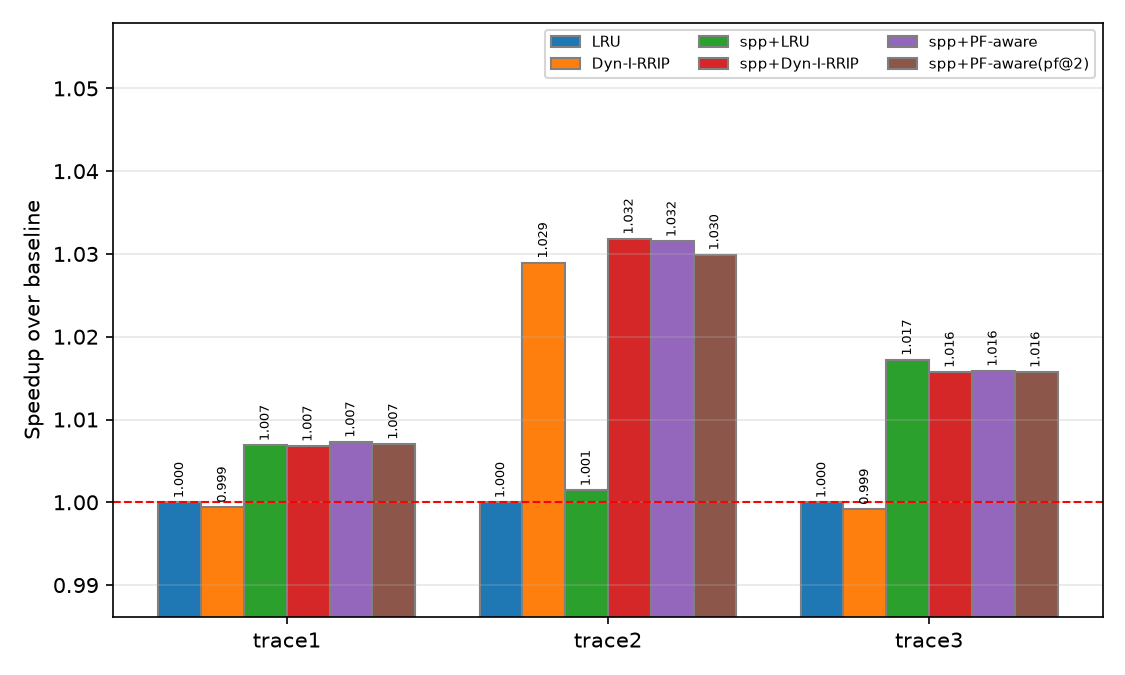
\includegraphics[width=0.8\linewidth]{../plots/task3_spp_speedup.png}
\end{figure}
\begin{figure}[H]
\centering
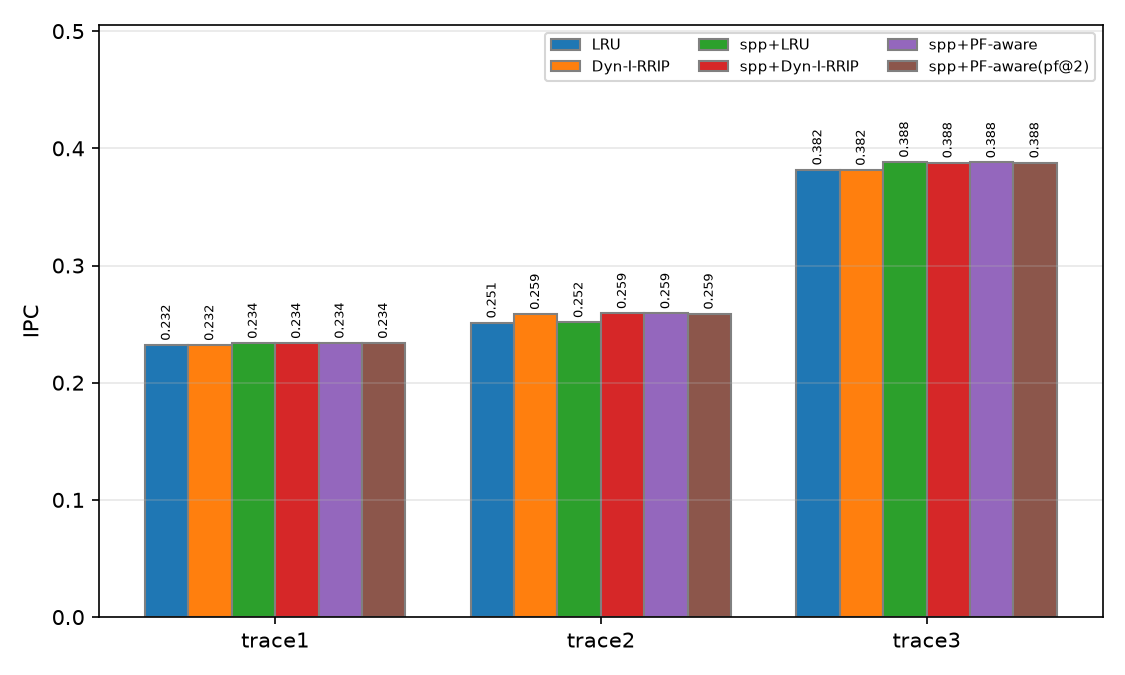
\includegraphics[width=0.8\linewidth]{../plots/task3_spp_ipc.png}
\end{figure}
\begin{figure}[H]
\centering
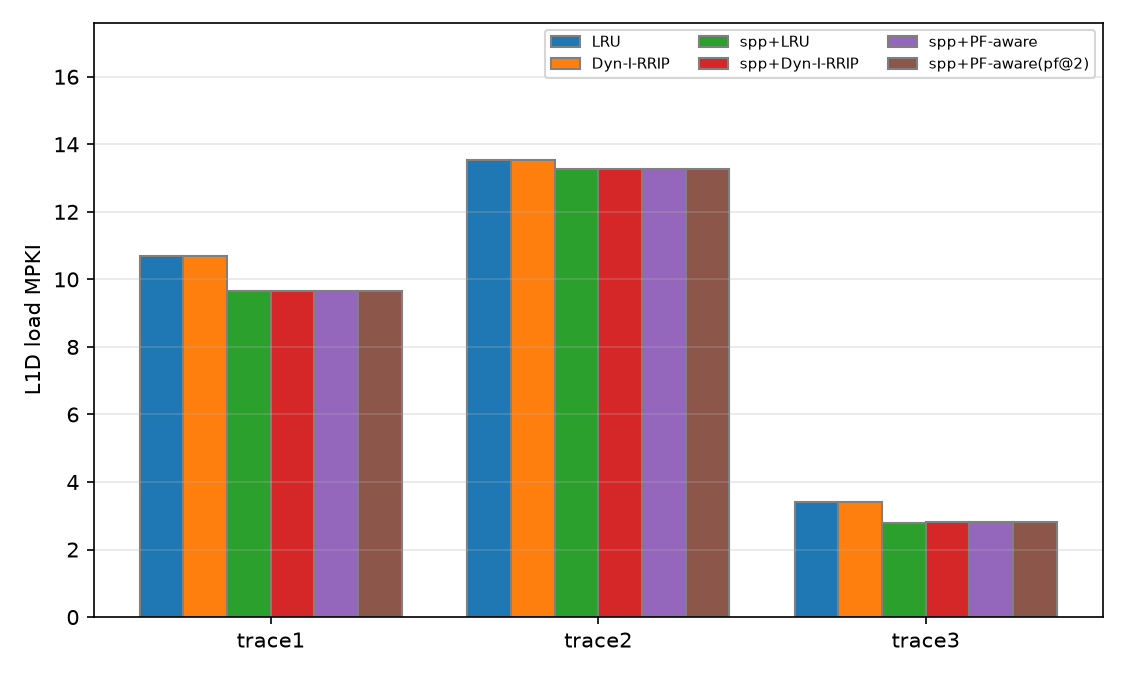
\includegraphics[width=0.8\linewidth]{../plots/task3_spp_l1d_load_mpki.png}
\end{figure}
\begin{figure}[H]
\centering
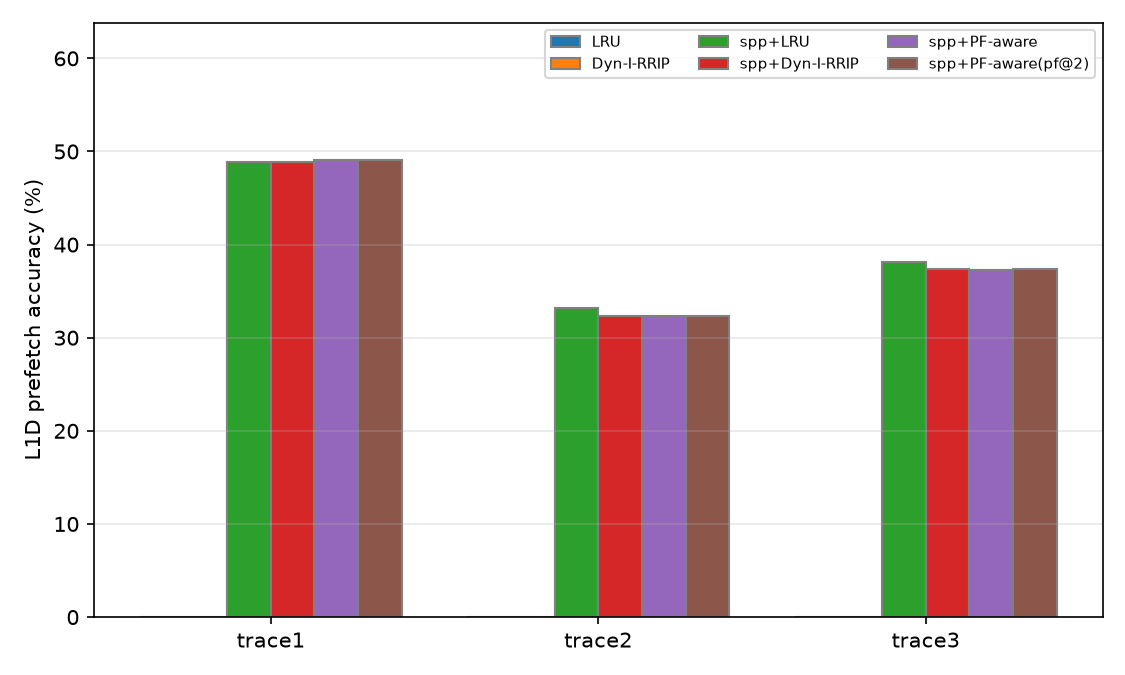
\includegraphics[width=0.8\linewidth]{../plots/task3_spp_l1d_pf_accuracy.png}
\end{figure}
\begin{figure}[H]
\centering
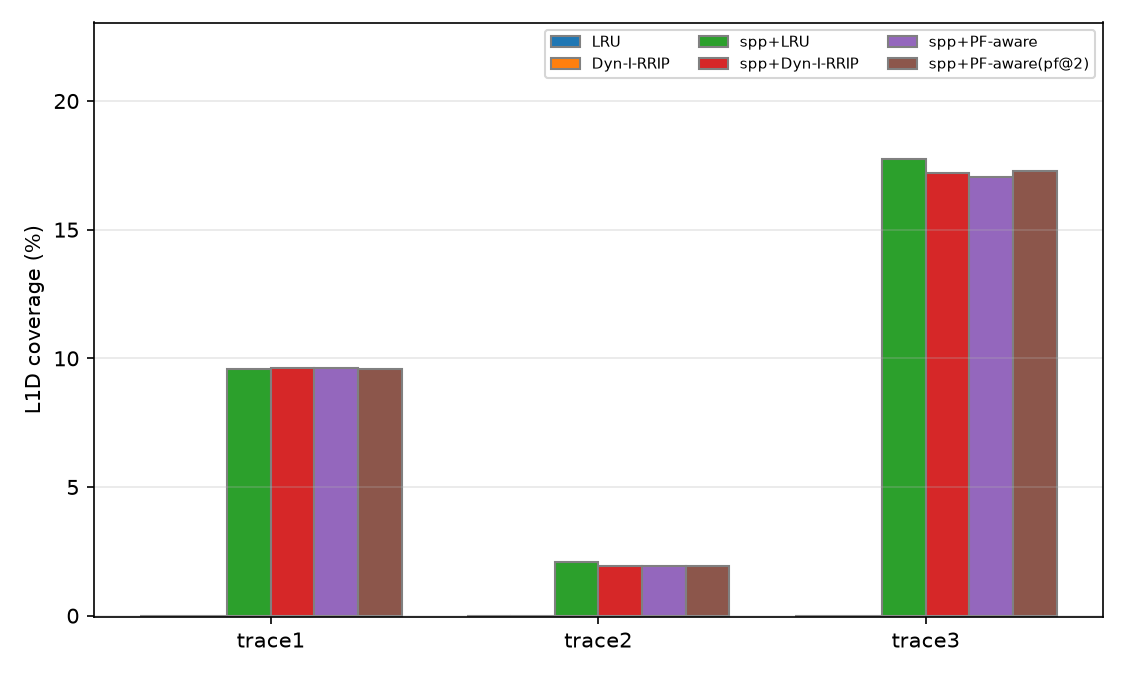
\includegraphics[width=0.8\linewidth]{../plots/task3_spp_l1d_coverage.png}
\end{figure}
\begin{figure}[H]
\centering
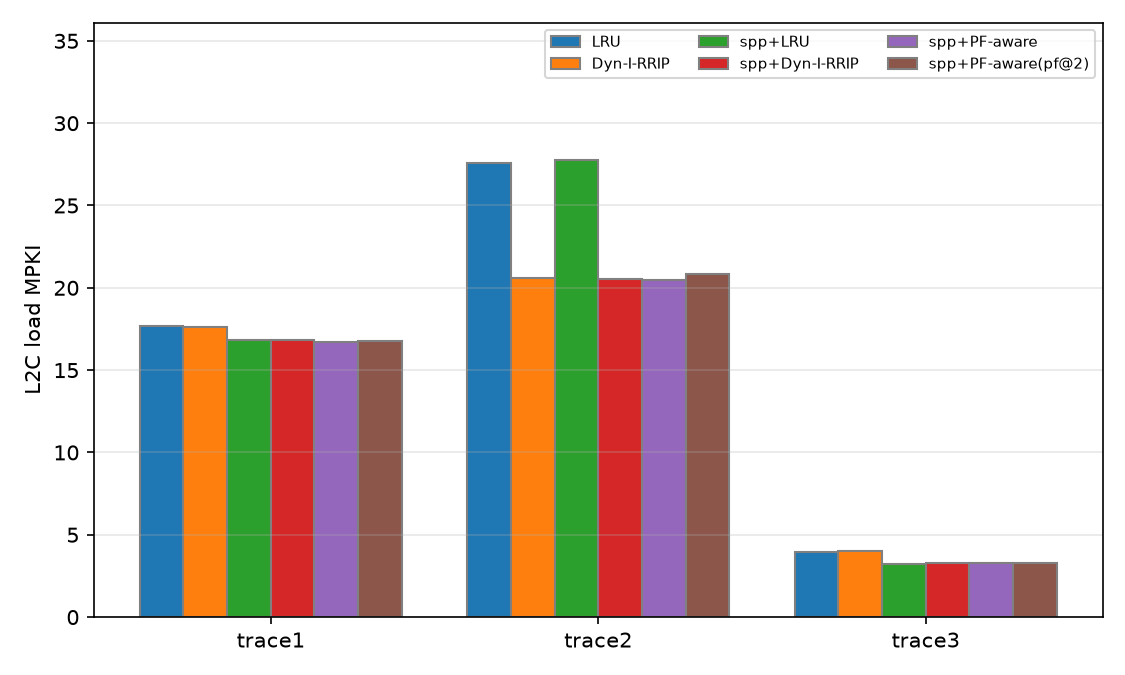
\includegraphics[width=0.8\linewidth]{../plots/task3_spp_l2c_load_mpki.png}
\end{figure}
\begin{figure}[H]
\centering
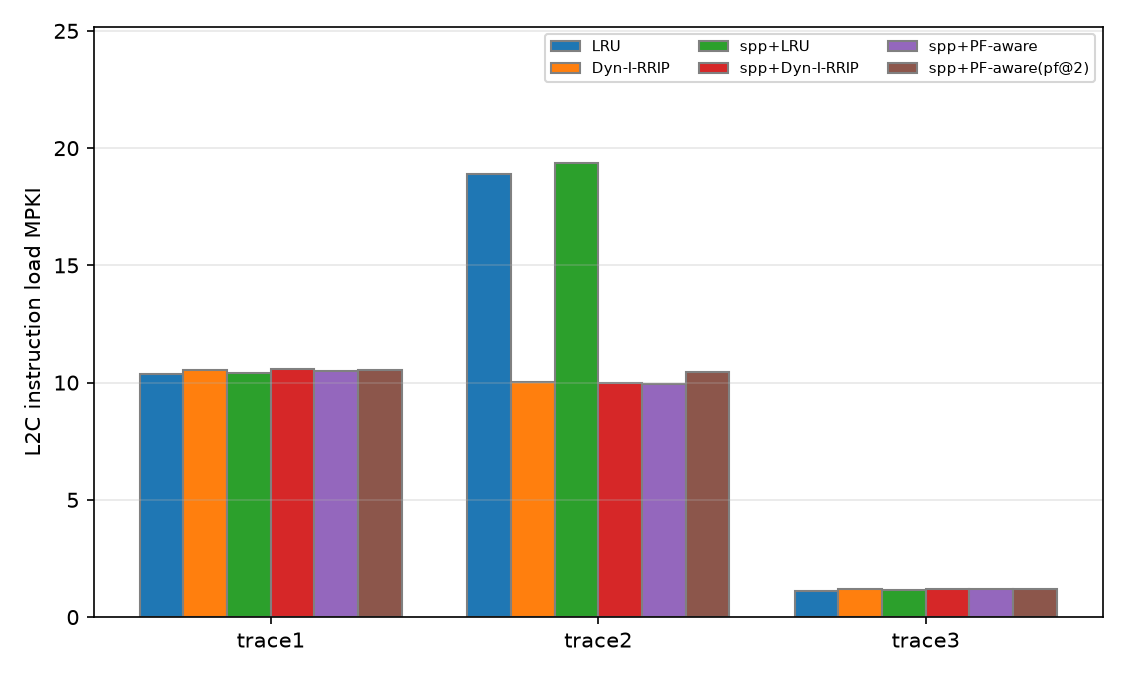
\includegraphics[width=0.8\linewidth]{../plots/task3_spp_l2c_instr_load_mpki.png}
\end{figure}
\begin{figure}[H]
\centering
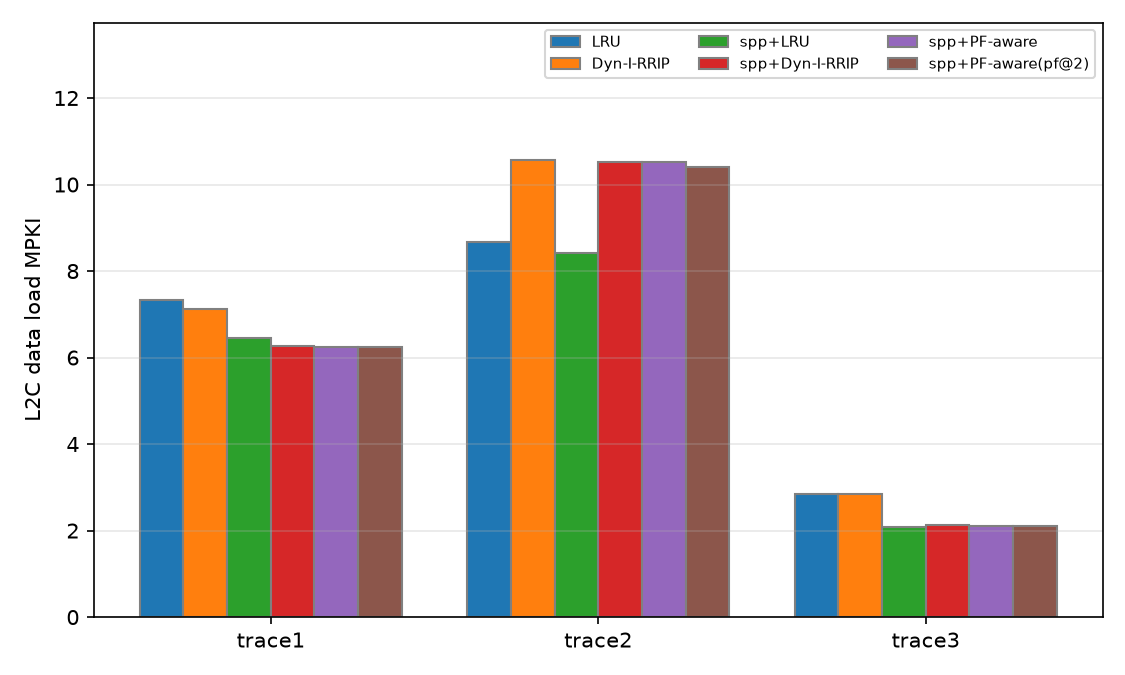
\includegraphics[width=0.8\linewidth]{../plots/task3_spp_l2c_data_load_mpki.png}
\end{figure}


\begin{itemize}
\tightlist
\item With SPP + prefetch-aware Dynamic I-RRIP we're getting a geomean of 1.0182, beating both Dynamic I-RRIP alone (1.0091) and SPP alone (1.0085).
\item The two gains add up: SPP cuts data misses at the L1D, and Dynamic I-RRIP cuts instruction misses at the L2 (trace2: L2 instruction MPKI 19.4 $\rightarrow$ 10.0).
\item Per trace, it's beating both on trace1 and trace2. On trace3 it's 0.13\% below SPP+LRU (1.0159 vs 1.0172), because the duel keeps trace3 in SRRIP mode (99.9\% of follower fills), and SRRIP itself is below LRU on trace3 (0.07\% without prefetching).
\item Prefetch awareness on top of the dynamic policy gives the lowest L2 MPKI on trace1/trace2, +0.05\% IPC on trace1, +0.02\% on trace3 and -0.03\% on trace2. The effect is this small because only \textasciitilde{}75-105K prefetch fills reach the L2C over a run, and SPP's throttle is already keeping them fairly accurate.
\item Inserting prefetches at 2 instead of 3 (-pf2) is worse on every trace (trace2: 1.0299 vs 1.0315), since the prefetches then compete with code and raise L2 instruction MPKI (9.96 $\rightarrow$ 10.44).
\end{itemize}
\end{document}
